%% Se lect the dissertation mode on
% See the documentation for more information about the available class options
% If you give option 'draft' or 'draft*', the draft mode is set on
\documentclass[dissertation,math,vertlayout]{aaltoseries}
\usepackage[utf8]{inputenc}

% TODO: remove
\usepackage{todonotes}

\usepackage{xspace} % for \setype
\usepackage{graphicx}
\usepackage{caption}
\usepackage{subcaption}
\usepackage{rotating}

\usepackage{url}
\def\UrlBreaks{\do\/\do-\do_}
\usepackage{breakurl}

\usepackage[withpage]{acronym}

\usepackage{hyperref}
\hypersetup{
	breaklinks,
    pdfpagemode={UseOutlines},
    bookmarksopen,
    pdfstartview={FitH},
    colorlinks,
    linkcolor={blue},
    citecolor={red},
    urlcolor={blue}
}

% Set the document languages
\usepackage[finnish,english]{babel}
\usepackage{amsmath,amssymb,amsthm}
\interdisplaylinepenalty=2500 % after amsmath to restore bad page breaks in the middle of equations
 % Adjust math line spacing
\renewcommand*{\arraystretch}{1.2} % for array/matrix environments
\setlength{\jot}{8pt} % for split environment

\usepackage{listings}
\usepackage[indentfirst=false,vskip=3mm]{quoting}

\newcommand{\textbfit}[1]{{\textbf{\textit{#1}}\xspace}}
\newcommand{\setype}[1]{{\texttt{#1}\xspace}}
\newcommand{\intel}[0]{Intel{}\xspace}

% The author of the dissertation
\author{Elena Reshetova}
% The title of the thesis
\title{Mobile and Embedded Platform Security}

\begin{document}

\widowpenalty10000
\clubpenalty10000

%% The abstract of the dissertation in English
% Use this command!
\draftabstract{\lipsum[1-3]}
%%\chapter*{Mobile and Embedded Platform Security. Dissertation by Elena Reshetova.}


\section*{Abstract}
% 2500 - 3000 words with spaces

The number of various mobile and embedded devices around us is growing very rapidly. Nowadays they are employed in many areas, such as automotive, industry automation, healthcare, smart home systems etc. At the same time, the number of attacks targeting these devices and associated infrastructure is also growing. The long history of information and device protection in the PC world has developed a set of hardware and software mechanisms, commonly refereed as \textit{platform security}, to withstand these attacks. However, they are usually not very well suited for mobile and embedded devices. As a result new platform security architectures for mobile and embedded device platforms were designed and widely employed. 

In this dissertation, we present a platform security model for mobile devices and compare various popular mobile platform security architectures with regards to this model. We also introduce a platform security model for embedded devices with the focus on the mainline Linux kernel due to its widespread use and popularity. Next, we outline the two major platform security aspects that nowadays present an ongoing challenge for mobile and embedded security architects: \textit{application isolation} and \textit{operating system kernel hardening}.   

Traditionally various mandatory access control (MAC) mechanisms have been used to achieve strong application and process isolation for personal computers and servers. Nowadays, these mechanisms (albeit with modifications) are making their way into mobile and embedded platform security architectures, such as SEAndroid MAC, used on Android mobile devices. This dissertation studies the challenges in adopting SEAndroid MAC for mobile devices, and presents the number of tools that can help security architects and researchers to create better SEAndroid access control policies. In addition, we also explore an emerging alternative method for application and process isolation, OS-level virtualization, and examine its security guarantees and shortcomings. 

The central piece of any platform security architecture is the security of the operating system's kernel, because its breach almost always leads to a compromise of the whole system. The designers of many popular mobile and embedded operating systems have spent considerable effort tightening the security of userspace applications and, as a result, attackers are more and more focusing their effort on the kernel itself. This dissertation examines the strength of existing protection in on of the Linux kernel subsystem, just-in-time (JIT) compiler for Berkeley Packet Filter, and shows that it is vulnerable to JIT spray attacks. Next, it considers the problem of temporal and spatial memory safety in the mainline Linux kernel and implements two different methods to address it.   

As a result, this dissertation addresses a number of important practical challenges in the present-day mobile and embedded platform security architectures and also gives a brief outlook on the upcoming future research directions in this area.  



% Let's add another one in Finnish
%\draftabstract[finnish]{\lipsum[4-6]}
% And yet another one in Swedish
%\draftabstract[swedish]{\lipsum[7-9]}

%% Preface
% If you write this somewhere else than in Helsinki, use the optional location.
\begin{preface}[Sipoo]

This dissertation is a result of the long learning journey from my internship and work at Nokia Research Center, Nokia Research and Development (R\&D), Intel Open Source Technology Center and my doctoral studies at the Department of Computer Science in Aalto University School of Science. I have been extremely lucky to work with and learn from many people on this journey, and I am grateful to each of them for the chance to grow my competence, skills and knowledge. 

I am more than grateful to my supervisor, Professor N. Asokan, for his excellent guidance, continuous support, enormous patience and encouragement through all these years. This dissertation would not have been possible otherwise. 

I am also grateful to my past and present work team leaders, Janne Mantyla, Ryan Ware and Deneen Dock for their support and understanding. Additionally I would like to thank all other people that have contributed to this work. Professor Tuomas Aura, for the start of my doctoral studies at the Aalto University. My co-authors, Kari Kostiainen, Jan-Erik Ekberg, Filippo Bonazzi, Thomas Nyman, Ravishankar Borgaonkar, Janne Karhunen, Hans Liljestrand, and Andrew Paverd. Linux Security community and especially Kees Cook, William Roberts and Daniel Borkmann, for giving valuable inputs and guidance for the kernel hardening and SEAndroid work. My pre-examiners, Dr. Alastair Beresford and Dr. Sven Bugiel, for their thorough reviews, valuable feedback and suggestions. Mustafa Masood, for his useful feedback and English correction on drafts of this dissertation. And lastly, Dr. Michael Steiner, for the honor of having him as the opponent for my dissertation. This work also has been supported in part by the Intel Collaborative Research Institute for Secure Computing at Aalto University.

Finally, I would like to thank my family and my husband, Janne, for their support and love on this long learning journey. 
\end{preface}

%% Table of contents of the dissertation
\clearpage
\tableofcontents

% To be defined before generating list of publications. Leave off if no acknowledgement
%\languagecheck{the Institute of Language Checks}

\listofpublications

\chapter*{Other Publications}%
\addcontentsline{toc}{chapter}{Other Publications}%
The following publications are not included in this dissertation.
\begin{enumerate}%
		\setcounter{enumi}{6}
		\renewcommand{\labelenumi}{\bfseries\Roman{enumi}}%
		  \item Li, Bo and Reshetova, Elena and Aura, Tuomas. Symbian OS Platform Security Model, \textit{The ;login journal, issue: 
Volume 35, Number 4}, August 2010
			\item Asokan, N. and Dmitrienko, Alexandra and Nagy, Marcin and Reshetova, Elena and Sadeghi, Ahmad-Reza and Schneider, Thomas and Stelle, Stanislaus. CrowdShare: Secure Mobile Resource Sharing, \textit{Applied Cryptography and Network Security}, June 2013
			\item Asokan, N. and Davi, Lucas and Dmitrienko, Alexandra and Heuser, Stephan and Kostiainen, Kari and Reshetova, Elena and Sadeghi, Ahmad-Reza. Mobile Platform Security, Synthesis Lectures on Information Security, Privacy, and Trust, \textit{Morgan \& Claypool Publishers}, December 2013
			\item McCool, Michael and Reshetova, Elena. Distributed Security Risks and Opportunities in the W3C Web of Things, \textit{NDSS Workshop on Decentralized IoT Security and Standards}, February 2018
\end{enumerate}%
		
%\clearpage

\chapter*{List of Abbreviations}
\addcontentsline{toc}{chapter}{List of Abbreviations}%
\begin{acronym}
\acro{AC}{Access Control}
\acro{AOSP}{Android Open Source Project}
\acro{API}{Application Programming Interface}
\acro{BPF}{Berkeley Packet Filter}
\acro{BYOD}{Bring Your Own Device}
\acro{CPU}{Central processing unit}
\acro{CVE}{Common Vulnerabilities and Exposures}
\acro{DAC}{Discretionary Access Control}
\acro{DRAM}{Dynamic Random Access Memory}
\acro{EVM}{Extended Verification Module}
\acro{GCC}{GNU Compiler Collection}
\acro{IMA}{Integrity Measurement Architecture}
\acro{IoT}{Internet of Things}
\acro{IPC}{Inter Process Communication}
\acro{JIT}{Just-in-Time Compiler}
\acro{HW}{Hardware}
\acro{KASLR}{Kernel Address Space Layout Randomization}
\acro{KCM}{Kernel Connection Multiplexer}
\acro{KPTI}{Kernel Page-Table Isolation}
\acro{KSPP}{Kernel Self Protection Project}
\acro{KVM}{Kernel Virtual Machine}
\acro{LSM}{Linux Security Module}
\acro{MAC}{Mandatory Access Control}
\acro{MPX}{Memory Protection Extensions}
\acro{MPXK}{Memory Protection Extensions for Kernel}
\acro{OEM}{Original Equipment Manufacturer}
\acro{OS}{Operating System}
\acro{PC}{Personal Computer}
\acro{ROP}{Return-Oriented Programming}
\acro{TCPA}{Trusted Computing Platform Alliance}
\acro{TEE}{Trusted Execution Environment}
\acro{TPM}{Trusted Platform Module}
\acro{UEFI}{Unified Extensible Firmware Interface}
\end{acronym}


\chapter{Introduction}
\label{sec:introduction}
\begin{quoting}
\todo[inline]{Find a nice quote here}
\end{quoting}

\section{Motivation}

Nowadays we are surrounded by enormous amount of various mobile and embedded devices on a daily basis: from smartphones and tablets to smart watches and smart glasses, from home entertainment and video surveillance systems to smart home appliances, from in-vehicle infotainment to flying drones. More and more functionality that used to be carried out manually by humans is automated with interconnected devices. Many recent attacks have shown that these devices and the associated infrastructure is very vulnerable to different types of attacks, such as leak of private or confidential data, violation of privileges, denial-of-service and many others. 

The long history of information and device protection in PC world have developed a set of techniques in order to withstand these attacks. The term "\textit{platform security}" is used to denote the set of security mechanisms implemented in a device against its pre-defined threat model. These mechanisms might provide run-time and offline confidentiality and integrity of devices and users data, prevent privilege escalation should a particular part of device become compromised, implement an anti-virus protection against malware, etc. However, the platform security architectures that have been originally developed for the relatively closed server and workstation systems are not well-suited for the mobile or embedded devices. 

Mobile devices, such as smartphones, were the first new wave of devices that required entirely different approach for designing platform security due to their open nature, i.e. ability for the user to install third-party applications, as well as a wide range of different user types (from very inexperienced ones to software developer hobbyists). A designer of the platform security solution could not anymore assume that a user of a device is an experienced system administrator understanding wide range of security risks and access control policy enforcing mechanisms. A mobile device user not only lacks this knowledge, but also in many cases is explicitly not willing to be involved in any such matters or decisions: he or she just wants to accomplish a simple task of sending a message or installing a popular game. The situation gets even more severe as we start looking into various in-vehicle infotainment systems where the user-driven open entertainment system might be partly co-located with the car instrument cluster with very strict safety requirements and regulations. 

The design and implementation of any platform security architecture varies greatly based on target environment, use cases, device capabilities, cost factors and prioritized set of risks and threats. A lot of prior research both in the academia and the industry examines this problem from all different angles and aspects, but the practice shows that achieving a good balance is still hard: many attacks are published regularly that find holes or abuse different platform security mechanisms and lead to severe implications on user's privacy, overall safety, denial of service and others. The producers of the devices, OEMs, in turn are facing heavy pressure to deliver fast (due to very competitive pace of modern industry) while balancing with the security requirements of various involved stakeholders from the ordinary users to various legislation’s. Finding the right balance between the appropriate level of security, development effort and the end-user usability represents the main challenge that any platform security researchers or architects face on a daily basis. Therefore the success of the developed platform security architectures depends on how well this challenge is addressed.   

\section{Objectives}
\label{sec:Objectives}

The goal of this thesis is to look at different practical platform security challenges that modern mobile and embedded systems are facing today and will face in the near future. The thesis attempts to develop mechanisms and techniques that can help OEMs to deliver devices with the right balance of security, practical deployability and usability. In order to do this, we want to make sure that whenever a certain mechanism or solution is proposed, it satisfies the following requirements:

\begin{enumerate}
	\item \textbf{Security}. The proposed mechanism must provide sufficient security level for the given set of use cases. There is no aim of reaching a perfect security if it makes the solution too unpractical for deployment or fails to satisfy the below non-security-related requirements.      
	\item \textbf{Practical deployability}. A mechanism or technique that is hard to deploy in practice is of little use in the industry. Instead the end goal of each proposed measure should be its integration and practical use in the respective area of interest. While it is not always possible to achieve this goal, it must be shown that the proposed solution satisfies all the standard deployability requirements of the field, such as performance, development life cycle, scalability, etc.  
	\item \textbf{Usability}.	The solution must be easy to use and understand for an ordinary user of the system. Latter might not necessary mean the end user of a device, but can also be an application developer, an access control policy writer, a kernel subsystem maintainer etc. These users usually have very different knowledge base and backgrounds, but in order for a solution to be taken into use and used correctly, it is essential to meet the usability requirements of all its intended users. 
\end{enumerate}

\section{Outline}

This dissertation is based on the six original publications which are grouped into three main areas, all around various aspects of platform security. An additional Publication VII, greatly based on Publication I, is also referred in this thesis. 

The foundation of Chapter~\ref{sec:plat-sec} is a generic platform security model for mobile devices defined in Publications I and VII. Through the survey of six different platform security architectures for the most common mobile operating systems, they show that despite the differences in the implementations, all of these architectures follow the same design patterns and principles. Same trend is also visible for embedded devices, but with a major focus on the mainline Linux kernel security mechanisms due to ease of maintenance and cost reduction. Chapter~\ref{sec:plat-sec} also presents a generic platform security model for an embedded device based on the mainline Linux kernel security components and mechanisms and explains their high-level purpose. The chapter ends with a motivation for selecting the two specific focus areas for this dissertation, namely \textit{process and application isolation mechanisms} and \textit{OS kernel hardening}. The former area, despite being researched for decades, still presents one of the biggest practical challenges for security architects due to many different (and not excluding each other) mechanisms present in the mainline Linux kernel and with almost unlimited ways for their configuration. The latter area, that recently got a lot of attention in the Linux security community, is of utmost importance, since if OS kernel is compromised as a result of successful exploit attack, all its security mechanisms are rendered ineffective.

Chapter~\ref{sec:ac-policies} focuses on the process and application isolation methods employed by modern operating systems and encompasses Publications II, III and IV. Publication II studies the mandatory access control mechanism, SEAndroid~\cite{smalley12}, employed by the Android operating system at the moment when OEMs had to go through the challenge of learning how to create their access control policies. The publication shows the difficulties that they were facing when trying to create the correct policy for their newly added components, as well as the most common pitfalls. It also presents a list of practical tools that can help OEMs, developers and security researchers to create better access control policies, including one of such tools, \textit{SEAL}. Publication III presents another tool, \textit{SELint}, that was specifically developed to smoothly integrate into the OEMs development workflow. Next, Chapter~\ref{sec:ac-policies} takes a different angle and, using Publication IV, examines the relatively new popular method for process isolation that is based on the OS-level virtualization. While this technique is prominent and has been recently greatly improved, there are still gaps that prevent its usage as a full alternative of traditional mandatory access control mechanisms.

Chapter~\ref{sec:kernel-hardening} considers a very different challenge: the need to be able to have the core of an operating system, OS kernel, secured against the various attacks. This is a very important area, because an OS kernel is becoming more and more attractive target for the attackers due to both its high privileges and recent tightening of the userspace security. Publication V shows a powerful attack against a very commonly used Linux kernel subsystem, Just-In-Time (JIT) Compiler for Berkeley Packet Filter (BPF), which served as a motivator for a stricter hardening of this subsystem. In turn Publication VI proposes two methods for addressing the Linux Kernel OS memory safety and therefore preventing common Linux OS kernel vulnerabilities, such as various buffer overflows and use-after-frees. 

Finally, Chapter~\ref{sec:discussion} presents an overall evaluation of the methods proposed in this dissertation against the objectives set in Section~\ref{sec:Objectives} and attempts to give an outlook on the whole future mobile and platform security challenges. 


            

\chapter{Mobile and Embedded Platform Security}
\label{sec:plat-sec}

Nowadays the vast market of mobile and embedded devices is growing much faster than the traditional PC or server markets. With many more new use cases being implemented and researched, one can see an explosion in the number of devices, their security requirements and platform security mechanisms. In order not to get lost in this constantly evolving variety, it is important to define a \textit{generic platform security model} that can be used for classifying different types of security mechanisms and techniques, as well as compare platform security architectures between each other. 

\section{Mobile platform security}

Publication I (which was later expanded to a book~\cite{2013Asokan}) focuses on creating this platform security model and comparing existing mobile platform architectures based on it. At the time of writing, mobile platforms were the most prominent direction for OS platform security research and this explains the focus of the publications. The platform security model, defined in~\cite{2013Asokan}, is built on top of a set of common design patterns described in Publication I. These include hardware-assisted security mechanisms (secure boot, trusted execution environment, sealing and attestation, etc.) described in Section III of Publication I, as well as software-only security mechanisms (protection of application integrity, run-time access control and permission assignment etc.), described in Section VI of Publication I. The history of many of these design patterns go back some decades. They continue to be used in emerging platform security architecture designs. For example, the "\textit{measure-before-execute}" design principle that is a foundation of the secure boot mechanism is a robust method to ensure that the software boot chain is free from offline (potentially malicious) modifications. Moreover, the first efforts to define and use hardware-assisted security mechanisms in platform security designs go back to late 1990s when the Trusted Computing Platform Alliance (TCPA)~\cite{pearson2002} defined the first hardware-assisted elements for PCs.

There are four different mobile platforms that are discussed in Publication I: Symbian, Java ME, Android and MeeGo. This set is further extended to six in~\cite{2013Asokan} by adding iOS and Windows Phone to the comparison. All of these platforms are compared in terms of security mechanisms they support, both hardware-assisted and software-only. However, as history has shown, only two of these mobile OSes have managed to reach significant device volumes as of now (end 2017), namely Android and iOS (73.5\% and 19.9\% of mobile market share respectively~\cite{osshare}). Both of these platforms preserve their overall platform security models, described in Publications I and~\cite{2013Asokan}, and some valuable new security mechanisms have been added over time, as well as existing ones improved. 

The Android platform saw a major usage growth and strengthening of its Mandatory Access Control mechanism, SEAndroid~\cite{smalley12} (a variant of SELinux). Starting from Android 5.0, SEAndroid is mandatory for OEMs to use and enable in the enforcing mode. The Security Hardware (HW) API, previously limited to the secure storage functionality only, has now been fully changed to an extensive and powerful \textit{Trusty TEE API}~\cite{trusty} that can be used as an interface towards Security HW. Android has also started to support various device encryption methods~\cite{androidencr} in order to guarantee confidentiality of users' data: the full disk encryption and the file-based encryption were added in Android 5.0 and 7.0 releases, respectively. The newly added hardware-backed keystore, Keymaster~\cite{androidkeymaster}, allows applications to take advantage of various cryptographic primitives and have their keys securely stored by underneath. Since Android 7.0, Keymaster also supports \textit{key attestation} and \textit{version binding}, where it is possible to bind keys to a specific version of the OS or even a patch version. 

The iOS platform continues to use the TrustedBSD kernel-provided MAC mechanism for its access control, but the MAC policy has been greatly improved and became more fine-grained~\cite{iOS11}.  Now all applications, including third party ones, can use \textit{entitlements} (iOS term for AC permissions) to request an access to the platform features, such as iCloud, or user information. Applications can be also arranged into groups by its developers for easier data sharing. The encryption and data protection methods have also greatly evolved. Now the offline data protection can be done on a per-file basis by assigning a file to a predefined protection class, such as \textit{Complete Protection} that guarantees that a file cannot be decrypted unless users enters the unlock passcode~\cite{iOS11}. The same protection classes (albeit with distinct keys) are implemented for the credential items stored in the \textit{Key Chain}. In addition an \textit{Effaceable Storage} feature~\cite{iOS11} guarantees a secure data erasure from the device's persistent storage. 

\section{Embedded platform security}

As we extend our focus from mobile devices to the embedded and IoT world, the situation changes: there is no more a single software platform or OS that dominates this market. This is due to the very different nature of how embedded devices are designed and produced by OEMs, as well as to a much wider set of use cases that such devices must support, such as automation, automotive, healthcare etc. A typical embedded device is usually a single purpose device, for example a light sensor, garage door controller or a factory supervision drone, but depending on the purpose can have very different hardware and software stacks. For example, a device might need to interact with a user and therefore require a user interface or it might not need one at all. The same applies to other technology support, such as TCP/IP networking, Bluetooth, wireless, etc. Moreover, embedded devices differ greatly in their HW capabilities: from very low-end devices having only KB of memory to high-end devices no different from a typical mobile or PC platform.

Thus there is not a single ready-made OS that would serve as a good fit for all of these different purposes without causing an overhead of unnecessary components. Instead, in the embedded world, it is more common to use an "\textit{OS-building set}", such as the ones provided by Open Embedded~\cite{OE2017} or Yocto projects~\cite{yocto2017}. Such sets are usually based on the mainline Linux OS (with the exception of very low-end devices that are not capable of running Linux) in order to minimize the maintenance cost, because stable mainline Linux projects usually take good care of keeping their components up-to-date and functioning with the rest of the mainline Linux infrastructure, as well as doing various bug fixes and new feature requests. Using such an OS-building set allows even smaller OEMs to deliver their devices faster to the market, which is crucial for their business model. Thus in this dissertation we focus on the mainline Linux kernel and its components and leave the other smaller footprint OSes, such as Zephyr~\cite{zephyr} and NuttX~\cite{NuttX}, out of the scope. 

When it comes to security, the above trend means that the platform security architectures for embedded devices are mostly composed out of mainline Linux kernel security mechanisms that are used as building blocks to satisfy the set of security requirements for a concrete device. Some bigger OEMs might extend these mechanisms by adding their own private solutions, but it is not common due to the high price of maintaining such solutions outside of the rapidly changing mainline Linux kernel source code tree. Following the model presented in~\cite{2013Asokan}, Figure~\ref{fig:platsec} shows the platform security architecture model that is applicable for any embedded device that would only use the mainline Linux kernel components and might optionally have security HW support. This is currently more common for rather powerful and advanced devices, but as the cost of including the security HW in the platform would drop with time, one would see more and more middle-range devices having such features~\cite{marketresearch},~\cite{iothwsecurity}. 


\begin{figure}[t]
	\centering
		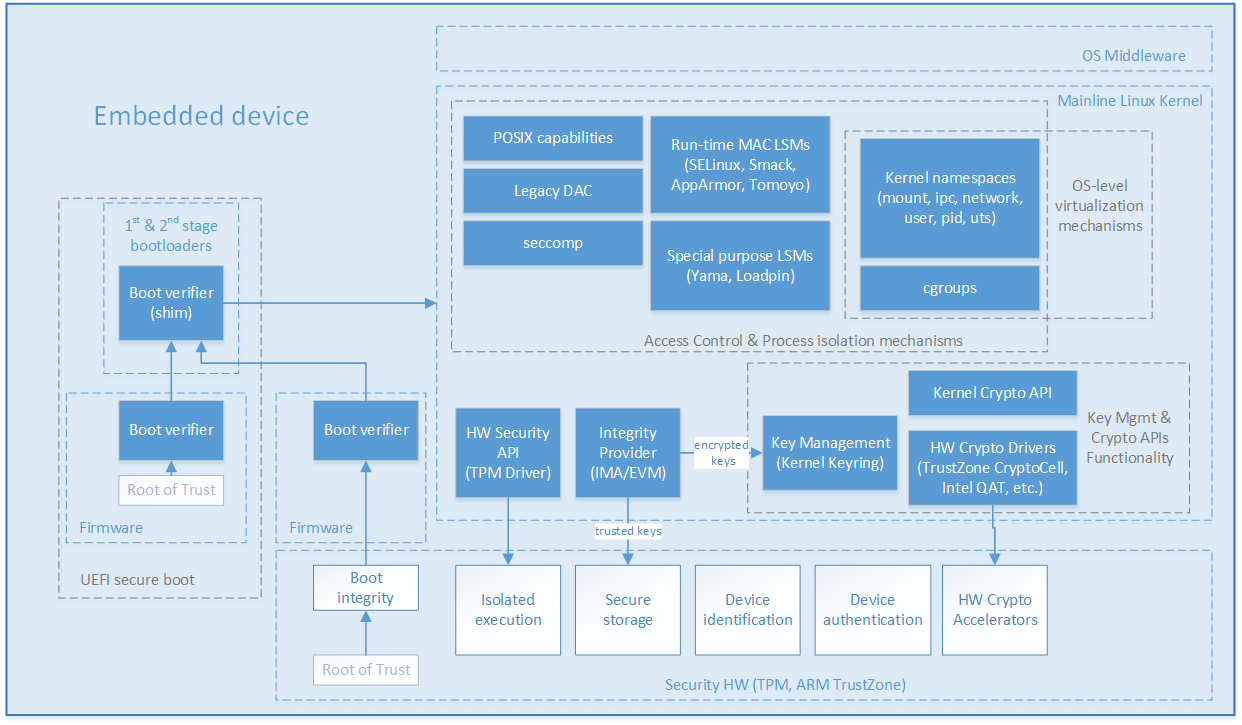
\includegraphics[width=1\textwidth]{figures/LinuxKernelPlatSecModel.png}
	\caption{Platform Security Model for an Embedded device based on mainline Linux}
	\label{fig:platsec}
\end{figure}

\subsection{Security HW and hardware-assisted mechanisms}

If present, the \textit{Security HW} layer can be implemented using many existing technologies, such as Trusted Platform Module (TPM)~\cite{tpm}, ARM TrustZone~\cite{trustzone}, etc. In order to communicate with this layer, one needs to provide a \textit{Security HW API}, which is usually done in the form of a custom Linux driver. For example, the mainline Linux kernel has a TPM driver~\cite{tpmdriver} that provides an API to perform various operations supported by TPM Security HW. Regardless of the particular implementation details, there is a set of common functionality that any typical Security HW provides:

\begin{itemize}
	\item \textbf{Root of trust}. \textbf{Secure boot} is used to guarantee that the device configuration (firmware and software) hasn't been altered from its original trusted state even when the device is in the offline state. This is typically done by measuring each component of the device firmware and software stack and comparing the measures to the signed reference values. Should the comparison fail, the boot can be either aborted (true "secure boot") or continued, but with some measures taken to protect the secrets residing inside Security HW ("authenticated boot"). However, in order for this system to work, one needs to start the measuring chain from an immutable \textbf{Root of trust} that is safely stored inside the Security HW layer\footnote{If present, the HW Root of Trust can be used for many other purposes in addition to the secure boot, such as derivation of keys, secure storage, etc.}. Alternatively, it is possible to implement the secure boot without the support of the security HW, like is done in the \textbf{UEFI Secure boot} mechanism~\cite{uefi}. In this case, the root of trust is embedded directly into the device firmware image.
	\item \textbf{Isolated execution} is another important functionality that is used to execute security-critical code that should not be observable in any way by potentially malicious OS or applications. This functionality is also commonly referred to as \textbf{trusted execution environment} (TEE).
	\item \textbf{Secure storage} functionality can be used by different OS components in order to guarantee data integrity and confidentiality even in the presence of offline attacks. For example, if a TPM module is present on a device, the Integrity Measurement Architecture (IMA) component~\cite{ima}, described below in more detail, uses TPM's secure storage functionality to guarantee security of its \textit{trusted keys}.
	\item \textbf{Device identification and authentication}. Embedded devices might need to have unique identifiers that can be used for different purposes, such as immutable MAC addresses, automotive identifiers, etc.  Additionally it should be possible for a device to reliably prove its identity to an external party, which is typically done in the form of a process called "\textit{remote attestation}". For example, this might be needed in order to get access to some external services or receive platform updates.
	\item \textbf{HW crypto accelerators} can be used in order to significantly speed up the costly cryptographic computations and in Linux are accessible via dedicated \textit{HW Crypto drivers}, such as TrustZone CryptoCell~\cite{cryptocell} or Intel Quick Assist Technology~\cite{intelQAT} cryptographic drivers.
\end{itemize}

The mainline Linux kernel also provides a \textbf{Key Management} (aka \textbf{Kernel Keyring}~\cite{keyrings}) and \textbf{Kernel Crypto API}~\cite{kernelcryptoapi} components. They can be used to generate and store keys and other credentials, and to perform various cryptographic operations, such as signing, encryption, hashing etc. The set of available algorithms consists of a set implemented within the kernel, as well as additional algorithms that might be provided by Security HW and exposed via \textit{HW Crypto Drivers} described above.

The last remaining mechanism, \textbf{Integrity Measurement Architecture} (IMA)~\cite{ima}, and its extension, \textbf{Extended Verification Module} (EVM)~\cite{ima}, can be used to extend the secure boot and guarantee the offline integrity of the userspace layer and filesystem. IMA/EVM does this by calculating a hash over each file before it is accessed and comparing this hash with a reference value stored in the file's signed extended attributes. IMA/EVM supports two types of keys: \textit{trusted} and \textit{encrypted}. The former depend on Security HW (such as TPM) being present on the system and stored within its secure storage facilities, while the latter ones can always be used and stored in the Kernel Keyring component. 

\subsection{Mechanisms for process isolation and access control}

The mainline Linux kernel itself has a number of platform security mechanisms that aim at addressing different security requirements. The biggest group of such mechanisms provides ways for implementing \textit{process and application isolation} on a device by means of a run-time access control. These mechanisms differ greatly in the level and type of access control they provide, depending not only on the mechanism itself, but also on its associated policy or configuration:

\begin{itemize}
	\item \textbf{POSIX capabilities}~\cite{caps} is a set of permissions that can be granted to a process in order to perform a defined system function. For example, a \setype{CAP\_NET\_ADMIN} capability allows a process to perform various privileged network-related operations, like administration of network interfaces and routing tables, access to advanced socket configuration settings, etc. By default the Linux superuser ("root" user with user id 0) possesses all defined capabilities, while other users have none, but it is possible to create different configurations using the \textit{file capabilities} feature~\cite{filecaps}. 
	\item The \textbf{Legacy Discretionary Access Control (DAC) mechanism}, initially developed decades ago for separating different device users and their data, is still present and functioning as originally designed, but since most present-day devices are single-user, it is used instead for separating processes and groups of processes. For example, the Android mobile OS uses Linux DAC mechanisms for implementing its permission model. The main downside of DAC is the lack of a centralized access control policy that can be enforced device-wise, because each data owner can freely grant access to its data to other processes. 
	\item The shortcoming of DAC is addressed by \textbf{Mandatory Access Control (MAC)} mechanisms that in the mainline Linux kernel are implemented in the form of \textit{Linux Security Modules (LSM)}, such as SELinux~\cite{smalley2001implementing}, AppArmor~\cite{bauer2006paranoid}, Smack~\cite{bauer2006paranoid} and Tomoyo~\cite{tomoyo}. They allow defining a unified access control policy for the whole device that can be formally analyzed for allowed information flows, conflicts, etc. MAC LSMs are very powerful access control mechanisms in Linux and are actively used on systems with strict security requirements for run-time process isolation, such as enterprise servers and mobile devices. 
	\item In addition to MAC LSMs, the mainline Linux kernel has \textbf{special-purpose LSMs}, Yama~\cite{yama} and Loadpin~\cite{loadpin}, that do not provide a system-wide MAC mechanism, but instead serve a much narrower focus of limiting process abilities. For example, Yama LSM allows limiting the dangerous Linux process tracing feature, where a (potentially compromised) process can examine the memory and running state of any other process running under the same user identifier. 
	\item \textbf{Seccomp}~\cite{seccomp2016} is another special purpose mechanism that allows a process to restrict the ability to make system calls to a smaller set specified using a seccomp filter. This can be useful if a process performs few system calls after the initialization stage and, should it get compromised later on, the compromised process abilities are significantly limited.
\end{itemize} 

Recently two additional mechanisms, initially developed to support OS-level process virtualization, have started to be used for application isolation on Linux: \textbf{Kernel namespaces}~\cite{biederman2006} and \textbf{cgroups}~\cite{cgroupsv2}. These mechanisms, described in more detail in Section~\ref{sec:os-virt} of this dissertation, allow a process to have its own limited virtualized view of the system to which it is confined and cannot escape from. However, there is a constant debate in the Linux security community about the security level that these mechanisms provide and the appropriate way of using them.   

\section{Discussion}

Out of all platform security mechanisms described above, the process and application isolation methods are ultimately the hardest ones to configure and use correctly. Not only does the mainline Linux kernel have multiple options that can be used simultaneously, but each of these options provides unlimited ways of how it can be configured. This is very challenging given that the end security of such mechanisms fully depends on their configuration or policy, which might be at best provided only in a reference policy form and only for certain limited use cases. For example, there is a SELinux reference policy for Fedora desktop that only covers the packages included in the Fedora distribution, but as soon as new packages are added or substituted (common in the case of embedded devices), the policy needs adjustments and additions. 

Therefore the first main focus of the dissertation, described in Chapter~\ref{sec:ac-policies}, is the method for process isolation and access control, where we will take a look at the typical challenges of building secure MAC policies, as well as propose methods and tools that can help in the process. We will also focus on alternative mechanisms for achieving process and application isolation by using OS-level virtualization methods. 

In addition to the mechanisms described above, there is an area that has recently gained a lot of attention in the mainline Linux security community, namely the OS kernel's protection against run-time exploits. The importance of this direction cannot be underestimated since a successful attack on the OS kernel itself renders all of its security mechanisms ineffective and useless. Therefore the second main focus of the dissertation, described in Chapter~\ref{sec:kernel-hardening}, is OS kernel hardening, where we will discuss the overall ways to enhance the run-time exploit protection of the mainline Linux kernel, as well as present concrete mechanisms for achieving this goal. 
  


\chapter{Process isolation and access control policies}
\label{sec:ac-policies}

The notion of access control and application/process isolation is one of the oldest in the history of information security with early pioneering work in the 1970s~\cite{saltzer75, Denning76}. Initially the main goal of access control methods was to isolate different users, with different levels of access, to the system assets, but as computers and other IT devices are increasingly single-user, the focus has shifted towards isolation of system processes and applications\footnote{In case a process or application becomes compromised, one wants to have the rest of the system and user's data protected.}.
 This trend was especially noticeable in various mobile platform security architectures, when users got the ability to install third-party software on their mobile devices: it required stricter isolation between the system's core platform and services (trusted set of entities) and user-installable services and applications (untrusted and potentially malicious).

A typical access control system can be viewed as a collection of one or more access control reference monitors that are consulted for access control decisions whenever any system access (such as operation on a filesystem object) is performed. The access control decision is done based on the access control policy for that access control reference monitor and defines if the access should be allowed or not. The access control policy is written in the form of access control rules that are defined in terms of \textit{subjects} (active entity performing the access), \textit{objects} (passive entity that is being accessed) and \textit{access types} (type of access attempted, such as read, write, etc.). Subject and objects are also typically grouped into a set of \textit{access control domains} using some identification or labeling scheme, allowing policy writers to arrange related and interconnected operating system (OS) components into logical blocks. Typically, most access control systems employ the principle that by default, any access is denied unless explicitly allowed by access control policy rules, or both the subject and object belong to the same access control domain.
 
Over the decades, the topic of process and application isolation has been the focus of a tremendous number of academic and industrial research: many systems and mechanisms have been proposed to address the challenges arising when designing and implementing access control systems. At a high level, these challenges can be arranged into the following categories that are all interconnected and affect each other: 

\begin{itemize}
	\item \textbf{Granularity.} One can design and deploy access control mechanisms with very different granularity levels following the principle of least privilege. On one side, one can place each individual process or even process thread into its own access control domain, and on the other side only create high-level access control domains that would isolate the trusted part of the system from user-installable and less trusted applications. It is clear that a fine-grained access control policy allows creating a more precise set of access control rules for a given access control object. However it usually directly negatively impacts other factors like manageability and performance, forcing access control policy's creators to search for some intermediate balance.
	\item \textbf{Manageability.} Most modern mobile and embedded OSes change at a high pace, with new system services and APIs introduced with each release, existing services fully redesigned, new use cases introduced, etc. The same applies to the system's access control policy: it must adapt and change with the OS to make sure it not only correctly reflects the current state of the system, but also correctly isolates and protects its entities. In addition, one needs to take into account how the OS is being developed. For example, if OS changes are done in a distributed fashion by different independent sets of development teams, the policy needs to be modular enough to allow changes to be performed relatively independently and in parallel. One just cannot assume that there is a single person that can manage all policy changes centrally.  
	\item \textbf{Performance.} Typically, an access control system is an integral part of an OS and for every system access, an access control decision needs to be made based on available parameters. This makes the runtime performance of access control mechanisms a critical consideration. It should be designed with care in order to make its overhead acceptable for the system as a whole.  
\end{itemize}

\textbf{Research questions:}   Section~\ref{sec:seandroid} of this dissertation attempts to answer the following research questions. \textbf{\textit{Access control deployment challenges}}, i.e. what are the challenges faced by designers of access control mechanisms in modern OSs in finding a balance among above three categories? The next research question is \textbf{\textit{practical tools for access control development and deployment}}, i.e. what tools or techniques can be helpful in practice to address these challenges? To answer these research questions, the dissertation selects one of the most popular mobile operating systems, Android, and its mandatory access control mechanism, SEAndroid~\cite{smalley12}, for a detailed evaluation as the most used mandatory access control mechanism on mobile Linux-based OSes. Another focus area of this dissertation is alternative ways in which process and application isolation can be done using various OS-level virtualization  techniques that have become a fashionable alternative to traditional access control mechanisms. Therefore Section~\ref{sec:os-virt} explores the \textit{\textbf{security of OS-level virtualization}} research question, i.e. whether this technique can provide a similar level of security as traditional mandatory access control mechanisms. 


\section{Mandatory access control on modern systems: SEAndroid}
\label{sec:seandroid}

Over the past decades, Android has become the most common OS for mobile devices. As the number of devices running Android has increased, so has the amount of malware targeting this operating system. Back in 2011, it became clear that the discretionary Android permission access control model is not able to provide the required level of security and work started on adapting the well-known desktop mandatory access control mechanism, SELinux, for Android OS. The resulting mechanism, SEAndroid~\cite{smalley12}, was largely based on SELinux, but contained some adjustments and additions required for supporting some Android-specific mechanisms, such as Binder Inter-Process Communication (IPC)~\cite{binder}. The biggest change was the SEAndroid reference policy, which was written from scratch due to significant differences between the Android and typical Linux desktop userspace layers, as well as a desire to have a small and compact policy. The initial policy and enforcement points were added to the Android 4.3 release back in 2012, but it wasn't until the release of Android 5.0 Lollipop that SEAndroid was required to be enabled on all devices in system-wide enforcing mode, which forced original equipment manufacturers (OEM) to implement SEAndroid policies. 

Traditionally, the way the Android ecosystem works is that Google delivers the reference code for the Android OS in the form of Android Open Source Project (AOSP)~\cite{aosp}. Next, this code is taken by different Android OEMs and customized at various levels including hardware adaption, new OEM-specific drivers and system services and new user facing applications. The reference SEAndroid policy, provided by the AOSP project, obviously does not cover these additions and customizations, and therefore OEMs need to adjust the provided SEAndroid policy, not only to get to a desired level of mandatory access control enforcement, but also merely to make their customized Android OS function correctly.

Publication II of this dissertation starts by examining eight different SEAndroid policies (taken from the Android 5.0 release) from various Android OEMs and presents an extensive analysis of these policies in terms of OEM-performed changes, policy size, complexity, etc. Table 1 from Publication II shows that all OEMs extensively modify the reference policy resulting in increases in overall policy size, as well as in the number of all other policy attributes and access control rules. Next, Publication II manually analyzes the characteristics of each of these eight policies and builds a set of typical pitfalls that OEMs make when making their policy additions. These include \textit{overuse of default types}, where many OEMs leave SEAndroid default labels\footnote{If an object is not given an explicit label by the SEAndroid policy, it is assigned one of the default labels, such as \setype{unlabeled}, \setype{device}, \setype{default\_prop}, etc.} for their newly added system objects. This typically leads to aggregation of large number of unrelated objects under a single default label and consequently violates the principle of least privilege: many different processes end up having legitimate access to the objects under default labels. Another typical pitfall is the \textit{aggregation of OEM-created applications under a few AOSP-predefined application domains}, such as \setype{platform\_app} or \setype{system\_app} instead of defining smaller, OEM-specific application domains. This leads to the enormous growth of such default domains (for example one OEM policy had 900 allow rules associated with \setype{system\_app} domain vs. 46 in the AOSP reference policy) and inability to prevent privilege escalation between different OEM applications placed in these domains. Other OEMs pitfalls include \textit{seemingly useless or forgotten rules} present in their policies, as well as \textit{rules that are dangerous for the overall security of the system} (such as granting access to rather sensitive parts of the system to untrusted domains). All of these pitfalls indicate that for the Android 5.0 release, OEMs struggled to deliver comprehensive and secure SEAndroid policies on their devices. 

\begin{figure}[t]
	\centering
		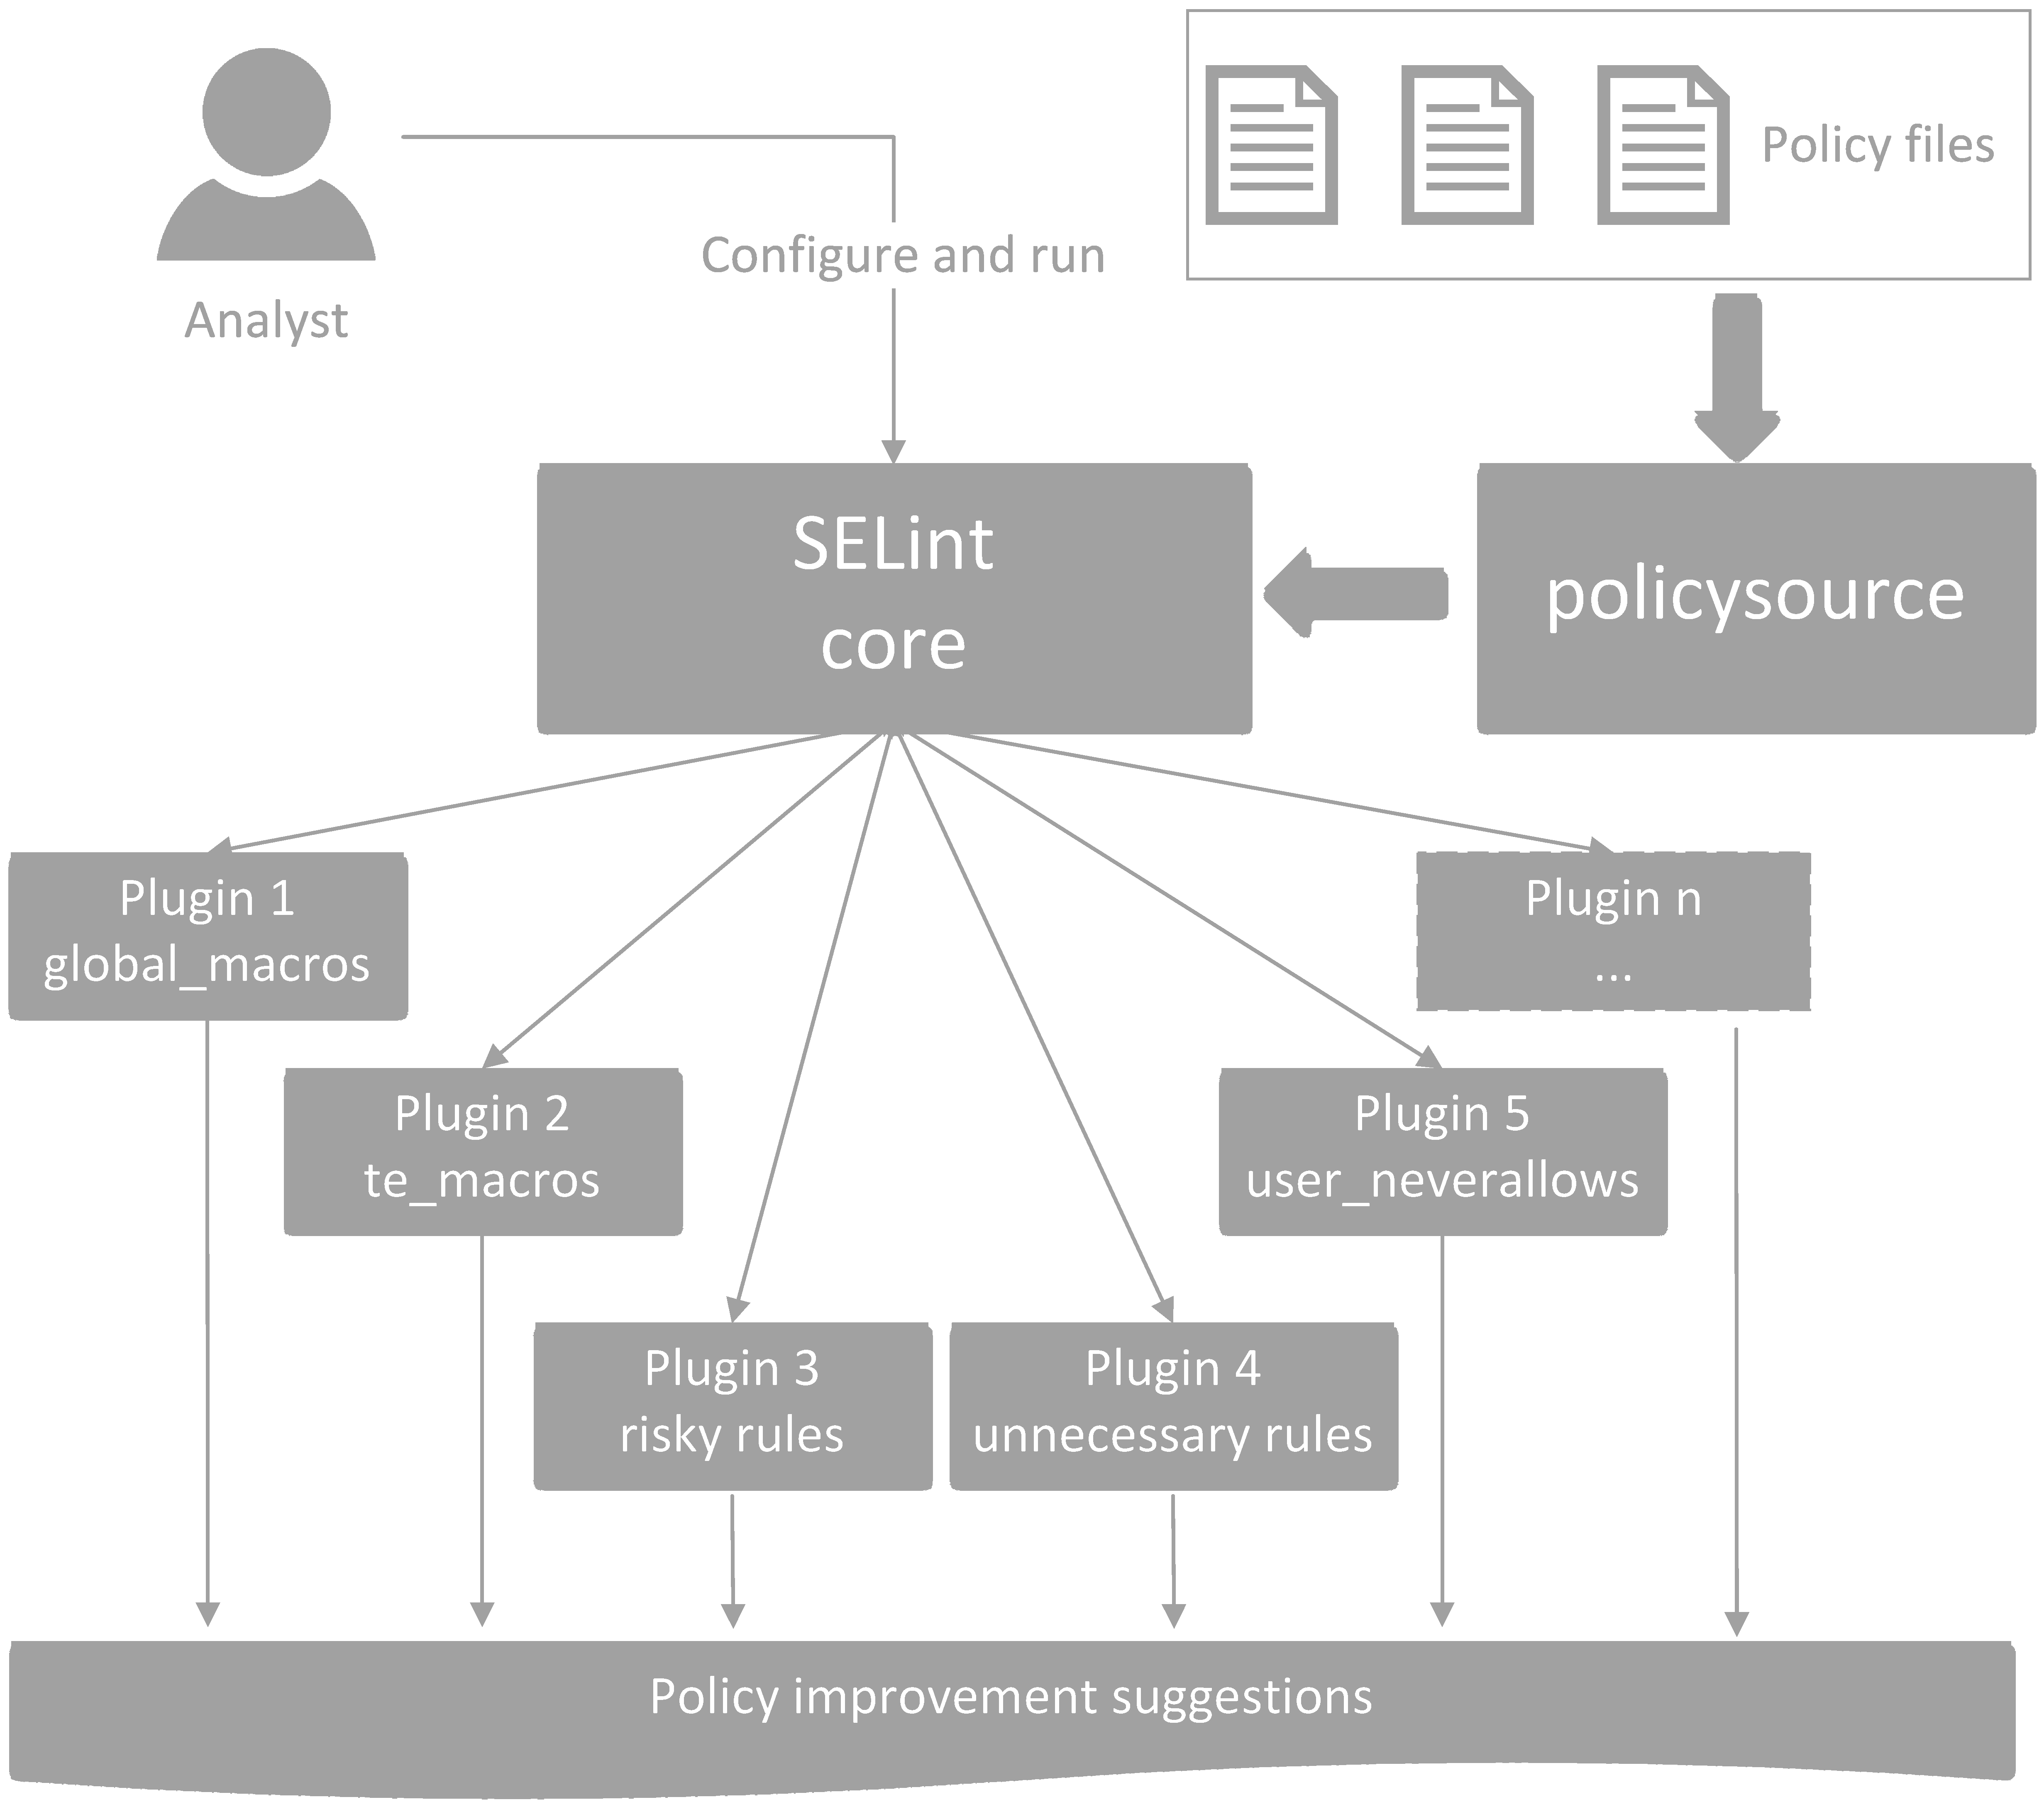
\includegraphics[width=0.80\textwidth]{figures/selint.png}
	\caption{The architecture of SELint (Adapted from Publication III)}
	\label{fig:selint}
\end{figure}

As a result of the above study, Publication II proposes a set of tools that should help both OEMs and security researchers develop better SEAndroid policies without the above-mentioned pitfalls, including various policy analyzers and visualization tools. It also implements one such tool, a live SEAndroid policy analyzer (SEAL), that performs different policy queries, not only based on the actual policy loaded on a device, but also also based on the run-time device state, i.e. running processes and services, filesystem labeling, etc. SEAL quickly obtains answers to various questions that an SEAndroid policy writer or analyst might have, such as "\textit{What files can a given running process access on a device?}" or "\textit{What processes can access a given object?}". This significantly simplifies debugging, troubleshooting and studying the given SEAndroid policy and gives a fast way to discover inconsistencies. 

Publication III presents the design and implementation of a more comprehensive SEAndroid tool, SELint, that provides a framework to improve SEAndroid policy development. It operates on the SEAndroid policy sources and allows smooth integration into the OEM policy development workflow. The architecture of SELint is shown in Figure~\ref{fig:selint}. It is composed from an SELint core, responsible for the processing of input SEAndroid policy files, and an initial set of SELint plugins that operate on a policy representation provided by the core and are able to perform policy analysis. The set of plugins are designed to be extensible and adapt to the needs of different OEMs or security researchers. The initial set of plugins includes: two plugins (\setype{global\_macros} and \setype{te\_macros}) verifying correctness of usage of different types of SEAndroid policy macros, a \setype{user\_neverallows} plugin that allows an OEM-specific verification of additional neverallow rules, an \setype{unnecessary\_rules} plugin that attempts to detect various ineffective rules\footnote{Some rules in SEAndroid policy are only effective in combination with others, such as domain transition rules when a process wants to transition its domain to a different one upon opening a certain type of object.} or rules used for debug purposes, and finally a \setype{risky\_rules} plugin that can be used to categorize SEAndroid access control domains into a set of related ones (untrusted, security-sensitive, core, etc.) and display various risk and trust relationships between them in a given policy. For example, it is possible to highlight the access control rules where the access to a security-sensitive object is given to a subject belonging to an untrusted domain.


\section{Application and process isolation using OS-level virtualization}
\label{sec:os-virt}

While traditional access control mechanisms and systems aiming for application and process isolation have existed for decades, recent years have seen the rise of an alternative approach, \textit{OS-level virtualization techniques}, widely known as "\textit{containers}". While originally developed purely to support various virtualization-based use cases, such as server consolidation or application and resource state management, they later on turned into various security-driven use cases, such as application isolation and the Bring Your Own Device (BYOD) scenario\footnote{A single physical device is used for both business and personal purposes that requires a strict isolation between these two environments and limited sharing.}. These additional focus areas brought new security requirements with respect to application and process isolation for OS-level virtualization techniques.

In contrast to the traditional virtualization solutions, like the well-known Xen hypervisor~\cite{xenproject} or Linux Kernel Virtual Machine (KVM)~\cite{kvmproject}, OS-level virtualization only virtualizes the OS kernel resources available to userspace, as opposed to the actual physical hardware resources, and therefore allows processes to share the same host OS kernel. This greatly reduces the performance overhead incurred by the OS-level virtualization and it consequently becomes possible to use this technology for efficient isolation of stand-alone applications or groups of applications. Despite its popularity, there is constant debate about the level of security that such virtualization provides in practice, as well as attempts to find flaws in the current implementation. 


\begin{figure}[t]
\centering
\begin{subfigure}{.5\textwidth}
  \centering
  \includegraphics[width=0.8\linewidth]{figures/os-virtualization-sys-model.png}
  \caption{System model}
  \label{fig:osv-1}
\end{subfigure}%
\begin{subfigure}{.5\textwidth}
  \centering
  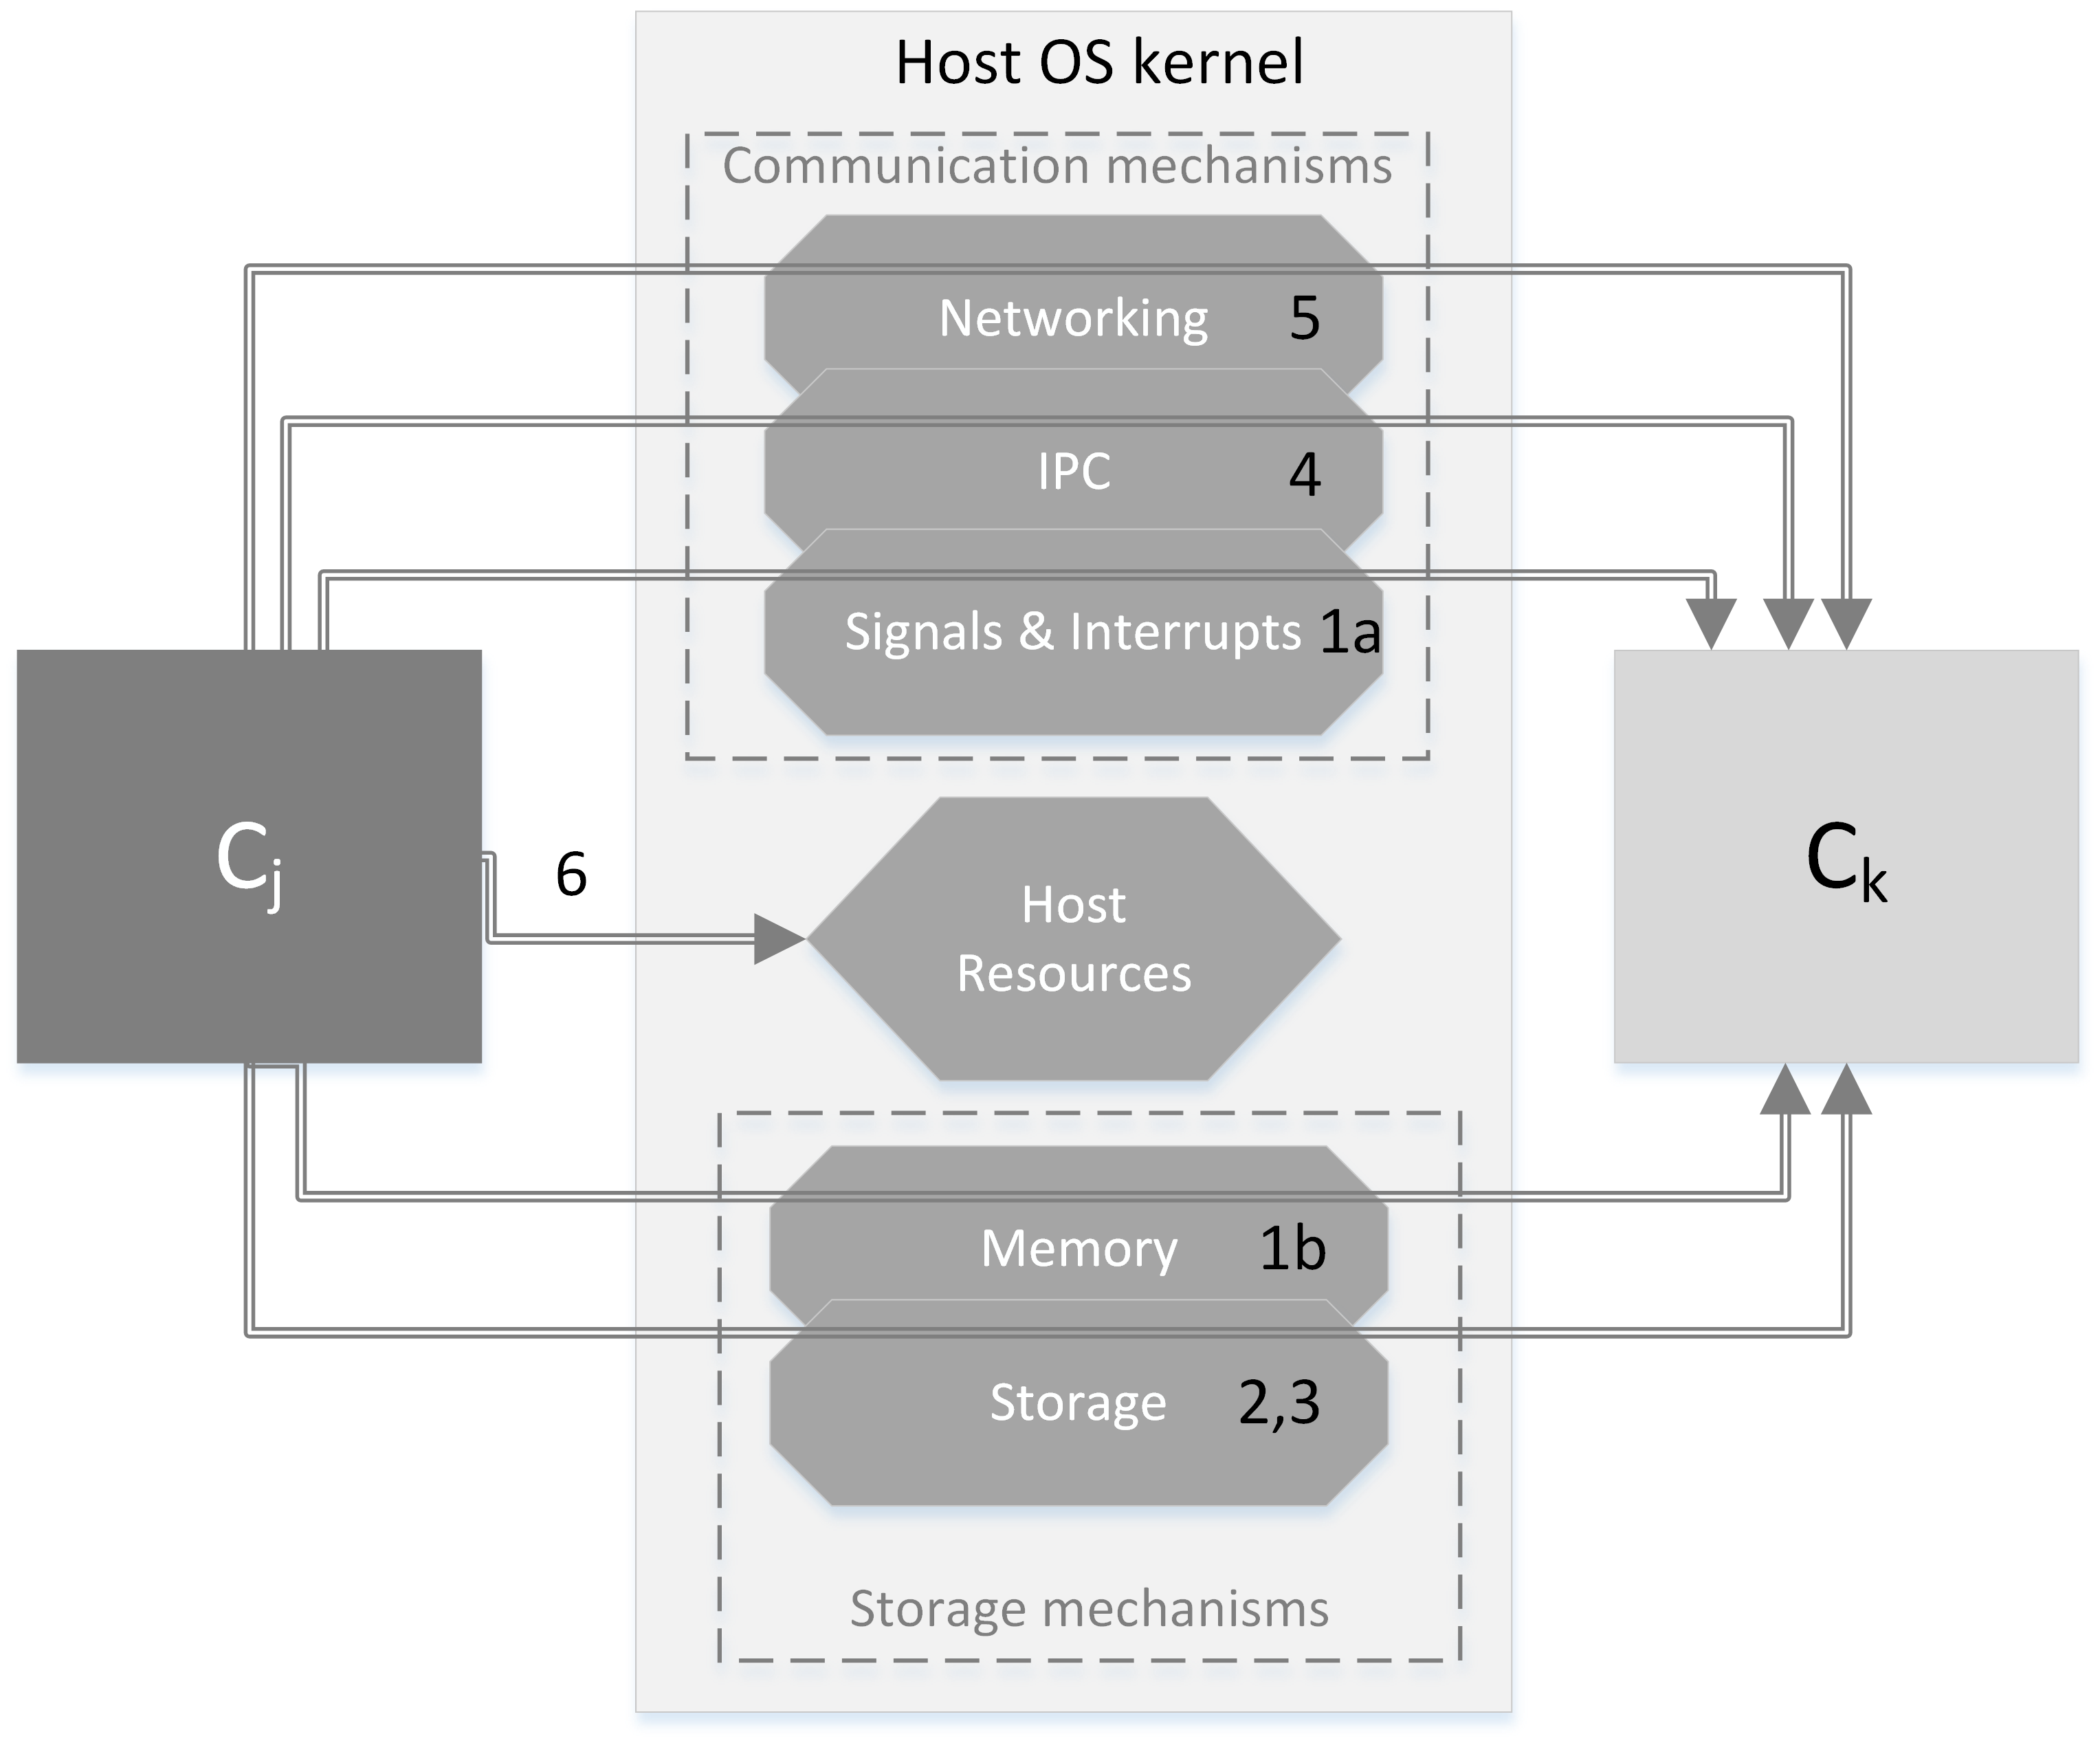
\includegraphics[width=1\linewidth]{figures/OS-virtualization-attacker-model.png}
  \caption{Attacker model}
  \label{fig:osv-2}
\end{subfigure}
\caption{OS-level virtualization. (Adapted from Publication IV)}
\label{fig:os-virtualization}
\end{figure}

Publication IV of this dissertation identifies the security requirements and generic model for a typical OS-level virtualization setup.
The system model for OS-level virtualization is shown in Figure~\ref{fig:osv-1}. The set of containers \setype{C\scriptsize{1}\normalsize..C\scriptsize{N}} is running on top of a shared host OS kernel and a userspace layer. The latter one can be either a minimal layer, only responsible for doing the setup of containers, or a full-fledged host OS userspace layer. The attacker model, shown in Figure~\ref{fig:osv-2}, assumes that an adversary has full control over a certain subset of containers (\setype{C\scriptsize{j}} in Figure~\ref{fig:osv-2}) and attempts to attack either another subset of legitimate containers (\setype{C\scriptsize{k}} in Figure~\ref{fig:osv-2}) running on the same host or the host OS itself. An attacker aims to achieve one of the following end goals: privilege escalation, legitimate container or host compromise or denial-of-service. This can be done by one of the attack groups 1 to 6 shown in Figure~\ref{fig:osv-2}, classified based on typical interfaces available to a UNIX-compliant OS. These attack groups are then converted into security requirements that each OS-level virtualization solution must fulfill in order to provide strong isolation guarantees: separation of processes, filesystem isolation, device isolation, IPC isolation, network isolation and resource management.   

Publication IV analyzes six different OS-level virtualization solutions against the above security requirements and outlines the differences in the provided level of isolation. It also summaries the state of OS-level virtualization in the mainline Linux kernel, implemented using "\textit{kernel namespaces}"~\cite{biederman2006}. A kernel namespace is a set of identifiers representing the global kernel resources, such as process and user ids, filesystem mounts, network interfaces, IPC objects, etc. A \textit{container} in the mainline Linux kernel is therefore a collection of such kernel namespaces that restrict visibility and communication between processes running in different kernel namespaces. In addition, Publication IV also defines a number of gaps that were limiting the usage of this technology in environments with strict security isolation requirements: the need for security namespaces, better support for resource management, etc. In recent years, progress has been made in closing these flaws and many new gaps have been identified. Below is a summary of recent changes to the mainline Linux kernel in the relevant areas that help improve OS-level virtualization in the mainline Linux kernel:  

\begin{itemize}
	\item \textbf{Security (LSM) namespaces.} Publication IV outlines the importance of security namespaces in order to be able to enforce independent mandatory access control security policies for different containers, as well as for the host OS. In recent years, this topic has received significant attention from the Linux kernel security community, with a number of mainstream Linux Security Modules (LSMs), such as Smack~\cite{smack} and AppArmor~\cite{bauer2006paranoid}, proposing their approaches and implementations~\cite{smackns},~\cite{apparmorns}. Unfortunately, these implementations are currently LSM-specific and only allow the creation of independent container-specific policies within the same LSM. However, this is a significant step forward and discussions on a unified solution continue.
	\item \textbf{Cgroups namespaces.} The cgroups kernel subsystem~\cite{cgroupsv2} is actively used in the mainline Linux kernel to implement resource management. It underwent a major change at the end of 2015 in an attempt to address various gaps and criticism from its users~\cite{rosen2016}. The new solution, cgroups v2~\cite{cgroupsv2}, added many new features, including namespace support for cgroups themselves. The latter allows independent cgroups hierarchies for different containers and restricts each container so it can only view its own cgroups rules. 
	\item \textbf{Automatic loading restriction support.} A process running inside a malicious container might try to use kernel features like automatic module loading as a way to escape the container. It can be done by requesting a kernel feature that is provided by a module that is not loaded in the kernel. In order to satisfy the request, the kernel would automatically load the module, despite the process having no permissions to ask about such an operation explicitly. In turn, this module can be potentially an old and vulnerable one, exposing the host OS kernel to attack. A recent proposal~\cite{harouni2017} to address this issue and create suitable controls has been discussed in the mainline Linux kernel community, and while the implementation details will still likely change, it is considered as an important security improvement. 
  \item \textbf{Keyring namespace support.} The mainline Linux kernel has a convenient facility, Kernel Keyring~\cite{keyrings}, for in-kernel storage and management of security keys and authentication tokens. The keys stored in these \textit{keyrings} are available not only for usage within the kernel itself, but also for userspace processes. From a security point of view, different containers and the host OS should naturally have separate kernel keyrings, but this hasn't yet been implemented in the mainline Linux kernel. Similar to other cases, an initial proposal~\cite{howells2016} by the keyring subsystem maintainer that separates keyrings between different user namespaces has been discussed by the Linux kernel security community and remains the expected future direction. 
	\item \textbf{IMA policy namespaces.} In addition to MAC mechanisms provided by various LSMs, the mainline Linux kernel has an Integrity Measurement Architecture (IMA)~\cite{ima} subsystem that aims to detect if files have been accidentally or maliciously modified when the device is in the offline state. This is done by calculating a reference hash value over the file content and attributes and comparing it to the newly calculated value every time the file is accessed. As is the case for LSMs, IMA operates on a policy that defines what files should be measured and when, as well as various exceptions. OS-level virtualization brings a similar requirement to IMA as for LSMs: the IMA policy needs to be namespaced in order to be able to support separate independent policies for the host OS and different containers. Active discussions on the best direction for IMA policy namespacing continue in the Linux kernel security community; the first implementation proposals have been presented~\cite{magalhaes2017}. 
	\item \textbf{Stricter handling of POSIX capabilities.} A very recent proposal~\cite{Bandewar2017} introduces a mechanism to limit the usage of POSIX capabilities~\cite{caps} inside user namespaces. This can be a very desirable feature for security hardening for OS-level virtualization since it is currently possible for a process that entered a user namespace to acquire a wide range of POSIX capabilities within this namespace and try to misuse them. 
\end{itemize}


\section{Discussion}

OS-level virtualization methods have gained a lot of attention and interest in the Linux community due to their ease-of-use. It is much easier to spawn a set of separate containers with independently running applications than achieving the same setup using MAC mechanisms. However, if sharing of data or IPC communication between these applications is required, then the setup quickly gets more complicated. Therefore our answer to the \textbf{\textit{security of OS-level virtualization}} research question is the following. While the implementation of the OS-level virtualization in the mainline Linux kernel continues to evolve and improve, the classical mandatory access control schemes are still required to provide the highest possible level of isolation, support fine-grained access control policies and minimize the security risks. Security architects must understand the details and the limitations of OS-level virtualization in order to make well-grounded choices on a set of isolation mechanisms for their systems in order to fulfill given security requirements. Publication IV of this dissertation presents a good model for such evaluation and comparison of available mechanisms, as well as guidance on identifying the missing isolation gaps. 

The SEAndroid MAC continues to be the main access control enforcement point of Android OS with all major OEMs now accustomed to the task of working with SEAndroid policies. The evaluation of initial SEAndroid policies, in Publication II, has answered the \textit{\textbf{access control deployment challenges}} research question by summarizing the main challenges and pitfalls of SEAndroid policy development and deployment. Publication II has also been crossed-referenced in the official Google SEAndroid documentation~\cite{seanroidsize}. Following the \textbf{\textit{practical tools for access control development and deployment}} research question, Publications II and III propose the SEAndroid tools, SEAL and SELint. These tools are being used by the Android community with numerous private forks on the project code trees and bug reports by the users once in a while\footnote{https://github.com/seandroid-analytics}. The SELint tool fulfills the main functional requirements defined in Section IV of Publication III by exhibiting an acceptable performance overhead, allowing its usage by ordinary users (after an initial expert configuration), being flexible and easy extensible. Due to the nature of SELint, i.e. the tool targets OEMs and internal use within their systems, it is hard to estimate on its usage in the real world, but a detailed evaluation of the tool can be found in Section V of Publication III. 

 

\chapter{OS Kernel Hardening}
\label{sec:kernel-hardening}
It is easy to see that a central piece of any platform security architecture is the security of the operating system (OS) kernel: any breach in this area almost always leads to the compromise of the whole system, especially if no security hardware support is present. This makes the OS kernel a very attractive target and many recent studies show that adversaries are more and more focusing their efforts on kernel-level attacks~\cite{stoep2016android}.\todo[inline]{put more references} This is especially true given that many popular mobile and embedded OSes spent considerable effort in tightening the security of their userspace applications and processes~\cite{stoep2016android}.\todo[inline]{put more references} For example, it used to be pretty common that many userspace daemons run with superuser privileges all the time making it very easy for attackers to obtain these privileges right after compromising a single userspace process. On the contrary, nowadays the privileges of each userspace application or daemon are minimized, and higher privileges are quite commonly even limited to the system or daemon startup time: after the initialization phase is finished, unnecessary privileges are dropped and cannot be misused by an attacker if the process gets compromised later on. Another common improvement is compartmentalization and isolation of the most vulnerable application parts, such as parsers and renderers, into separate sandboxed processes further reducing attacker's opportunities. As a result of these efforts, modern successful attacks on userspace applications are very complex and require chaining of multiple vulnerabilities in order to reach the desired result. In contrast a single vulnerability directly in the OS kernel provides an attacker with superuser privileges right away.

This thesis focuses on a specific OS kernel, namely the Linux kernel, due to its widespread adoption for mobile and embedded devices: more than 2 billion mobile devices were already running Android OS powered by the Linux kernel~\cite{googleio2017}, many embedded manufacturers build their OSes based on Open Embedded/Yocto~\cite{OE2017, yocto2017} projects with the Linux kernel at its base etc. 
In addition, the Linux kernel is developed fully in the open and any person is able to propose ideas or contribute the code to the mainline (of course assuming that the Linux kernel maintainers agree with the approach).

Past studies~\cite{stoep2016android, cooklss2016} show that the Linux kernel vulnerabilities have remarkably long life times. It takes on average five years between the time when a vulnerability is introduced into the kernel source code and the time it is fixed. Moreover even after it is finally fixed in the mainline Linux kernel, it is very difficult to estimate when the fix is delivered to the end devices: it might take anything between a number of days to a number of years. In addition some older embedded or mobile devices might actually never see these updates, making them perfect attack targets. Thomas et al.~\cite{Thomas2015}, in 2015, showed that on average 87.7\% of Android devices are exposed to at least 11 known critical vulnerabilities including the ones in the Android OS kernel itself. The time window between the public announcement of kernel vulnerability and its fix (usually pretty fast) in the mainline kernel and the time the fix is propagated to most of the devices is the period of golden opportunity for many attackers: all the details about the vulnerability is known and sometimes even proof-of-concept exploits can be obtained.

As adversaries have been turning towards attacking the Linux kernel itself, security architects, researchers and engineers have been exploring various methods for its better protection. A lot of the effort has been put into improving the overall testing suites for the Linux kernel, various static and dynamic code checkers are also used regularly and automated. New tools, including better commit verification scripts are being developed to assist developers, better code review practices are established etc. However, it is unrealistic to assume that it would ever be possible to have all the bugs in the source code found and fixed even in the well-maintained mainline Linux kernel. The situation is even worse for drivers and other non-mainline code developed by OEMs~\cite{stoep2016android}. Such code might get very limited code review, little testing and be written under harsh time-to-market requirements making it a good place for introducing bugs and vulnerabilities.

An alternative approach that defenders can take is to consider how modern kernel exploits are written and try to eliminate all attack paths that helps exploit writers to succeed. This is exactly the path that the Kernel Self Protection Project (KSPP)~\cite{kspp} has taken. KSPP is an open community of developers and security experts that aims to develop new or adapt existing kernel hardening measures for the mainline Linux kernel. 

Figure~\ref{fig:exploit-steps} shows how a typical attack on the Linux kernel is carried out. In Step 1 an attacker usually spends time to explore the target kernel offline in order to collect as much information about it as possible. This step is usually performed with high privileges and an attacker has a full access to the kernel memory layout, various debugging and tracing tools etc. Preventing this step is impossible due to the open nature of Linux operating system, but various protection methods can be employed to minimize the value of collected information. For example, Kernel Address Space Layout Randomization (KALSR)~\cite{cook2013} and other techniques such as GRKERNSEC\_RANDSTRUCT~\cite{randstruct2017} can make sure that every time a Linux kernel is loaded on the system, the memory locations of many of its components are randomized, and therefore an attacker cannot use the information collected during Step 1 to locate required kernel elements (modules, symbols, structures etc.) during the later steps of a run-time attack. 

\begin{figure}[t]
	\centering
		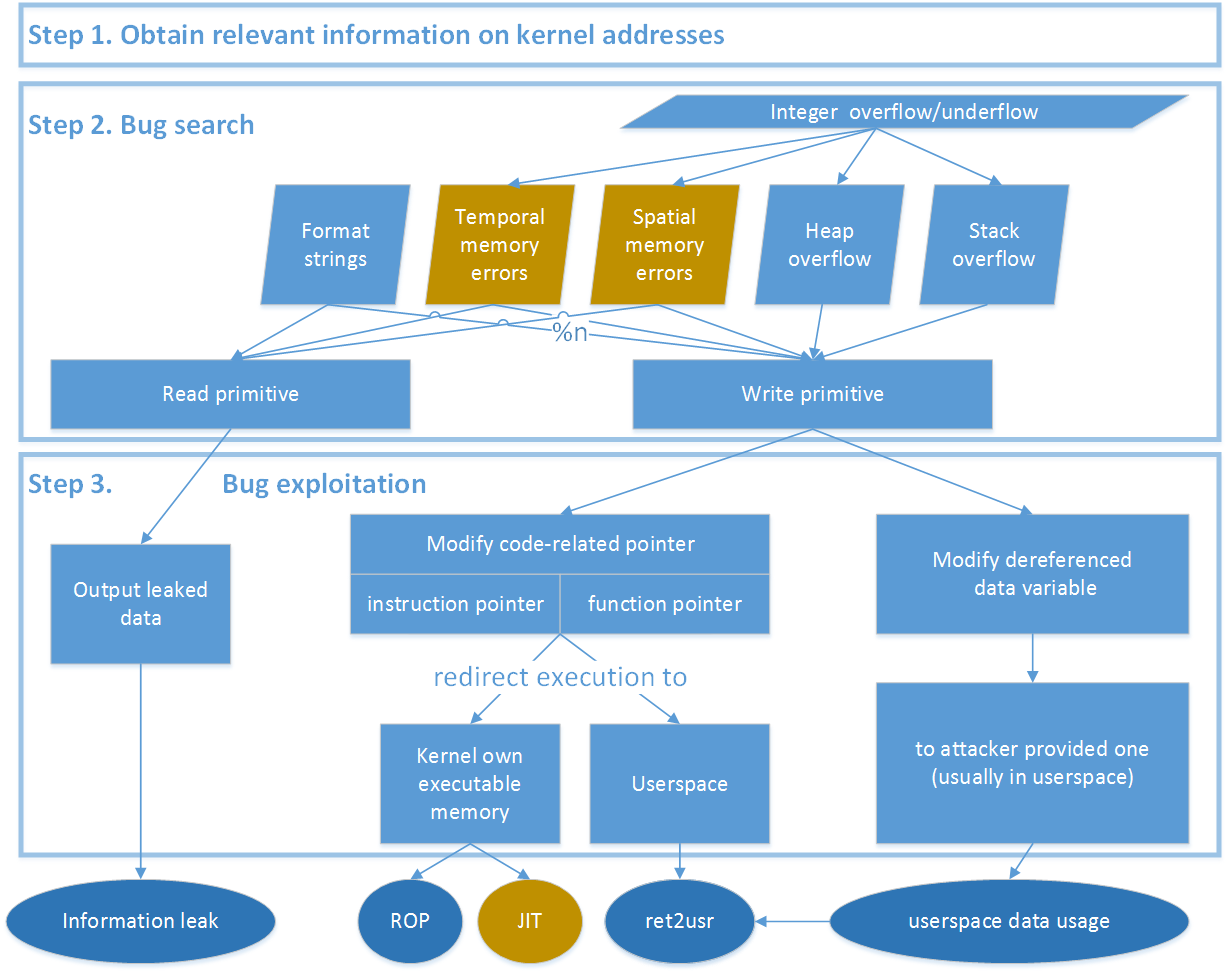
\includegraphics[width=1\textwidth]{figures/kernel_exploit_steps.png}
	\caption{High-level overview of a kernel attack}
	\label{fig:exploit-steps}
\end{figure}    

In Step 2 an attacker needs to find a suitable bug that would allow him to obtain a read or write primitive inside the Linux kernel. There are many bug classes that can be explored for this purpose and Figure~\ref{fig:exploit-steps} shows the most common ones for the Linux kernel. Some bug classes such as Heap and Stack overflows, typically lead to a write primitive, while some, like temporal and spatial memory errors (see Section~\ref{sec:kern-mem-safety} for definitions) can lead to both of them depending on the code where bug is present. The format string vulnerabilities typically lead to a write primitive, except in cases when format string is using \setype{\%n} specifier that allows writing input data to a pointer (and as a result a write primitive). Integer overflow/underflow bugs do not typically give a read or write primitive straight to an attacker, but they can be used to create other bug classes. For example, if an overflown integer is used to allocate a buffer, the resulting buffer is going to be of a smaller size than required leading to a buffer overflow bug (spatial memory error). Preventing Step 2 from happening would be an ideal case for defenders, but in reality it is very difficult and costly to prevent certain classes of bugs from fully happening. Nonetheless a lot of work is being done in this area within the KSPP project and Section~\ref{sec:kern-mem-safety} of this thesis looks into preventing a wide range of memory errors in the Linux kernel. 

Last in Step 3 an attacker can finalize the exploitation using the bug(s) found in Step 2. In case of a read primitive, the end result is usually a run-time kernel memory leak that can be either valuable on its own (various sensitive information, such as keys and credentials) or can be used as supporting information for launching further attack steps using another kernel bug. In turn, a write primitive can be used by an attacker to modify either a code-related pointer or a dereferencing of a kernel data pointer or structure. The code-related pointer can be either directly an instruction pointer (as it is the case with stack overflow attacks) or a function pointer located in places such as function pointer and descriptor tables. All of this would allow an attacker to redirect the execution flow to a desired place. That place can be either the kernel's own executable memory (by building and chaining the available attack gadgets in ROP-like technique or using mechanisms like just-in-time (JIT) compilers) or userspace (various \textit{ret2usr} attacks), where an attacker usually has more control over the memory layout and more mechanisms for continuing the attack and making it persistent over reboots. An attacker can also modify a data pointer (commonly to a structure located in the userspace) that might allow him to perform various data-only attacks. Many different protections can be put in place in order to prevent Step 3 from happening, but they are not generic and depend on the chosen attack path. For example in order to prevent a function pointer overwrite, function pointer tables can be made read-only after the kernel initialization step. Similarly in order to prevent a direct modification of an instruction stack pointer various return address protection techniques, such as stack canaries~\cite{edge2014}, guard pages~\cite{kstackoverflow2017} etc. can be employed.    

Within the KSPP project this thesis has investigated into two important areas of kernel hardening that are highlighted in orange in Figure~\ref{fig:exploit-steps}). The first one is preventing attackers from misusing the Berkeley Packet Filter (BPF) Just-In-Time (JIT) compiler in order to place the attack payload. The BPF JIT compiler is the only JIT compiler in the Linux kernel that executes programs supplied by unprivileged userspace, making it a very valuable target for the attackers.  The second area is the ability to prevent kernel memory errors, such as use-after-frees or buffer overflows, that can greatly affect the overall security of the Linux kernel and help eliminating many past and future vulnerabilities. The subsections below explain each aspect in more details as well as the contribution this thesis makes in addressing these two problem areas.  

\section{Security of Berkeley Packet Filter Just-In-Time compiler}
\label{sec:bpf-jit-attack}

Having an OS kernel mechanism with the ability to execute userspace-supplied code is always very attractive for attackers. 
The mainline Linux kernel has such a mechanism: the Berkeley Packet Filter (BPF)~\cite{kernelfilter2016} and the associated Just-In-Time (JIT) compiler, that is basically an in-kernel virtual machine available for unprivileged execution from userspace. Historically this mechanism was introduced to speed up packet filtering on networking sockets, but nowadays it is also used in a wide range of non-networking applications, including trace points~\cite{starovoitov2015}, syscalls filtering in seccomp~\cite{seccomp2016}, Kernel Connection Multiplexer (KCM)~\cite{corbet2015} etc. There is even a proposal to use BPF for creating a user-programmable Linux Security Module, Landlock~\cite{landlock2016}, that considerably widens the set of BPF use cases.

\begin{figure}[t]
	\centering
		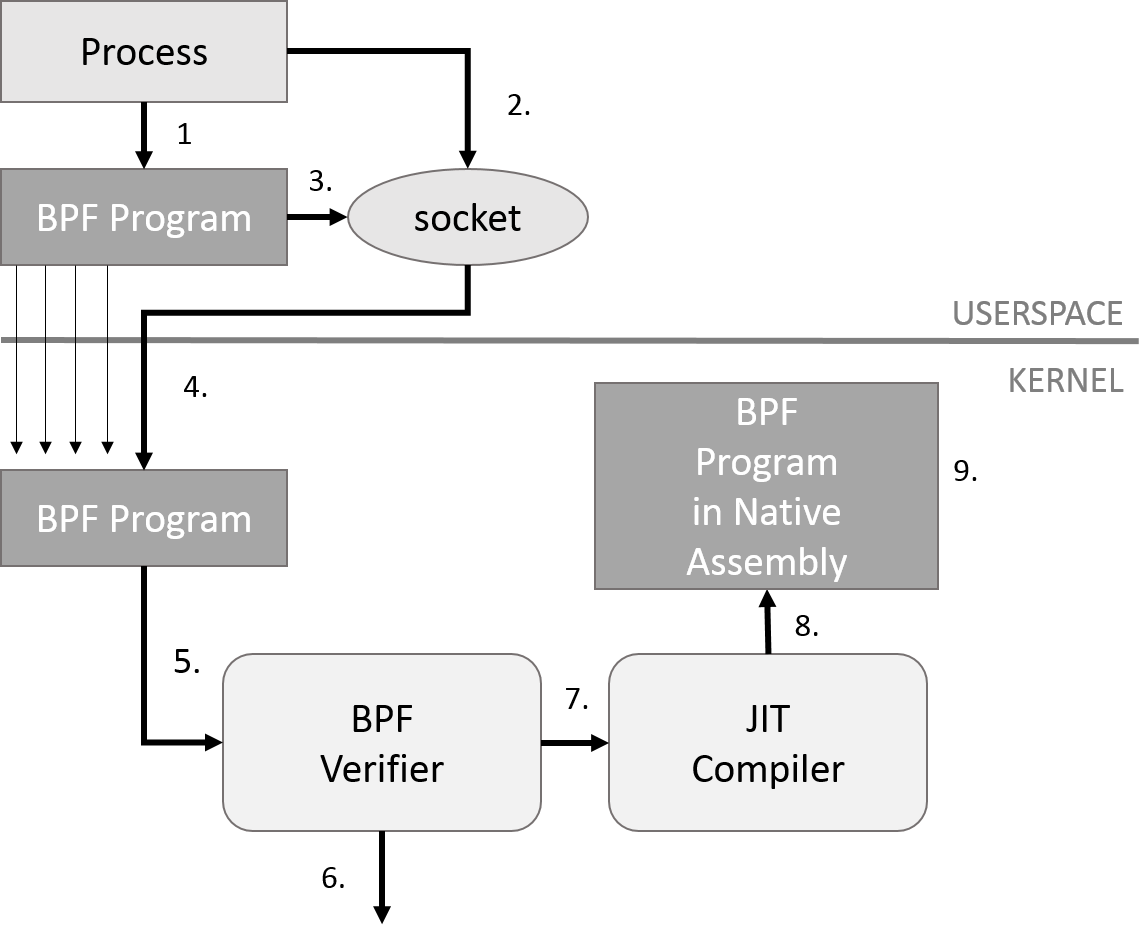
\includegraphics[width=0.80\textwidth]{figures/bpf-overview.png}
	\caption{Linux kernel Berkeley Packet Filter and JIT compiler (From Publication V)}
	\label{fig:bpf-overview}
\end{figure}

\todo[inline]{Remember to either get the copyright permission or modify the figure}          


The overall flow of how a BPF program is processed by the kernel is shown is shown in figure~\ref{fig:bpf-overview}.  
A userspace process expresses its packet filtering algorithm in a form of the BPF program that it wants to attach to a socket. A BPF program is written in the BPF interpreter language that can be executed by BPF in the kernel. When a BPF program is loaded to the kernel, it is first verified by a BPF Verifier component that attempts to check the correctness of supplied program. If the check passes, then the program is attached to the socket and will be executed every time the packet is received for that socket. For non-networking scenarios a BPF program will be executed every time a certain action is performed by its creator, i.e. for the seccomp system calls (syscalls) filtering, a BPF program will be invoked every time a process executes a syscall. In addition in order to further speed up the filtering, the BPF program can be given to the JIT compiler that translates it to native machine assembly language. This is typically enabled for high-performance networking use cases and disabled on a typical desktop system.  

The above flow can be abused to load the attacker-supplied payload into the kernel memory using an attack technique called \textit{JIT spraying}~\cite{blazakis2010, bania2010jit}. The original proof-of-concept exploit was done back in 2012~\cite{mcallister2012attacking} and showed that BPF JIT compiler design and implementation are very vulnerable to such attacks. As a result a protective measure was merged in the mainline kernel that attempted to randomize the start memory address within the page where the BPF program gets loaded and will the rest of the page with architecture-specific instructions (aka \"poisoned zone\") that would hang the machine fully if attacker tries to execute them. This made it really hard (with a probability of success of only about 0.0004\%) for an attacker to find supplied payload. However, the root cause of the problem, i.e. the ability to supply the attacker payload in BPF programs using constants, was not fixed at that time, despite the suggestions from some security experts\footnote{The Grsecurity kernel security project \url{grsecurity.net}}.

Publication V of this thesis analyzes the security issues of the BPF JIT compiler and builds a number of successful attacks on the latest (at that time) available mainline 4.4 Linux kernel despite the security fixes done in the past. 
Our best attack approach, described in Section 4.3 of publication V, analyzes how memory allocation for a BPF program happens and specifically how randomization of the start address is done in the mainline kernel implementation. 
This analysis discovered that for BPF programs of total size of PAGE\_SIZE - 128 - PROGRAM\_HEADER\_SIZE (size can be controlled by an attacker by adding more or less BPF instructions) the maximum size of the poisoned zone can be calculated in advance (equals to 128 bytes) and it allows an attacker to reliably jump over the poisoned zone and land securely on the BPF program payload. The resulting overall success rate for the attack is 99.6\%, which proves that much stronger security measures are required for the BPF JIT compiler in order to provide adequate security against JIT spray attacks. As a result of this work a number of mitigation measures were merged to the mainline kernel that eliminated possibility to perform this type of attacks\footnote{\url{git.kernel.org/cgit/linux/kernel/git/torvalds/linux.git/commit/?id=4f3446b}}. It is no longer possible to supply the attacker's payload in BPF programs using the constants due to the blinding process (XORing with a random number) done for each of them prior to its placement in the memory.

\section{Kernel memory safety}
\label{sec:kern-mem-safety}

Memory errors can be very dangerous for the security of OS kernel since they can give an attacker the ability to read or write kernel memory, which is normally inaccessible for a userspace process. The cause of these errors is the absence of inherent memory safety in C, which is the primary implementation language of the Linux kernel. 
Numerous past CVEs (CVE-2014-2851, CVE-2016-4558, CVE-2016-0728, CVE-2014-0196, CVE-2016-8440, CVE-2016-8459, and CVE-2017-7895) as well as vulnerability studies~\cite{raheja2016analysis, chen2011linux} show that memory errors are a big problem for the Linux kernel and needs addressing in order to be more robust against these attacks.

Typically memory errors are divided into two classes:

\begin{itemize}
	\item \textbf{Temporal memory errors} happen when pointers to uninitialized or freed memory are dereferenced. A typical example is a \emph{use-after-free} error when a memory that is dereferenced by the pointer has already been prematurely freed. Another example is a null pointer dereference errors, when an initialized pointer is attempt to being dereferenced. 
	\item \textbf{Spatial memory errors} occur when pointers are dereferenced outside the bounds of their intended areas. The most common example here is a buffer overflow when data is written past the end of the memory area allocated for the buffer. 
\end{itemize}

Memory safety has been researched for decades both in academia and industry.
Many solutions have been proposed to fully eliminate the root cause of the problem, but they are rarely used in practice due to the significant side effects they bring. 
The primary issue is usually the performance; most of the developed solutions~\cite{hastings1991purify},~\cite{patil1995efficient},~\cite{patil1997low},~\cite{nagarakatte2009softbound},~\cite{jones1997backwards},~\cite{yong2003protecting},~\cite{xu2004efficient},~\cite{nethercote2004bounds}, and ~\cite{dhurjati2006backwards} incur a significant and non-acceptable run-time performance overhead.
Other typical issues are lack of backwards compatibility~\cite{necula2002ccured},~\cite{grossman2005cyclone},~\cite{austin1994efficient} and the need to make source code changes~\cite{necula2002ccured},~\cite{grossman2005cyclone}. 
In addition, almost all existing mechanisms were developed for the userspace and have not been considered for in-kernel use with the exception of recently developed kCFI~\cite{Rigo} and KENALI~\cite{kenali}. However, even these systems have not been developed with the goal of merging them into the mainline Linux kernel and therefore exhibit some design choices, such as a requirement to have two compilation rounds, that won't be acceptable by the mainline kernel developers\footnote{\url{http://www.openwall.com/lists/kernel-hardening/2017/08/05/1}}. 

Publication VI of this dissertation takes a deep look at both temporal and spatial memory problems in the Linux kernel and proposes two practical measures that address each of these types of errors. 

\subsection{Preventing temporal memory errors for objects protected by a reference counter}
\label{sec:kern-mem-ref-count}

The lifetime of a shared object in the Linux kernel is typically managed using a \textbfit{reference counter}. 
Such a counter is incremented every time a reference to an object is taken and decremented when a reference is released. 
When the counter reaches zero the object can be safely deleted since there are no references to this object anymore (object is not used).

The above presents a simple logic, but practice and history of Linux kernel vulnerabilities (for example CVE-2014-2851, CVE-2016-4558, CVE-2016-0728, CVE-2017-7487 and CVE-2017-8925) shows that reference counting schemes are error prone. If a developer forgets to perform an increment or decrement in some code branch (quite often on a rarely exercised error-handling or exception path), it might lead to counter imbalance and as a result incorrect object lifetime handling, i.e. use-after-free situation on the object. This can be misused by attackers in order to construct efficient and simple kernel exploits: an attacker needs to allocate a different kernel object (but with a user-controlled content) from userspace over the same memory that is going to be mistakenly freed and then use the reference to the old object to trigger the code execution. One such example is the exploit based on kernel CVE-2016-0728\footnote{\url{https://www.exploit-db.com/exploits/39277/}}. The exploit abuses a bug inside the kernel keyring facility: forgotten decrement of the reference counter when attacker asks to substitute the session keyring with the exactly same keyring. 
The problem is even bigger given the fact that the current implementation of reference counters in the Linux mainline kernel allows a counter to overflow upon reaching its maximum value (specific to the architecture). 

The first part of the publication VI analyzes how developers have used reference counters in the Linux kernel and describes the design of a new reference counter data type \setype{refcount\_t} and its API that prevents reference counter overflows by its internal design. 
The new type is specifically designed for the reference counting use only and therefore has a much more limited API compared to the generic type, \setype{atomic\_t}, which is used for reference counters but also for many other purposes. This allows to reduce potential development errors when implementing reference counters and improves the code review process.   
This type and respective API have been accepted into the mainline Linux kernel and are becoming the de-facto standard for implementing reference counters. 
Paper VI also presents an overall kernel-wide analysis and conversion of existing reference counters to \setype{refcount\_t} that resulted into more than 170 accepted patches\todo[inline]{update exact number since it is changing all the time}. The analysis was done using a static analyzer, Coccinelle~\cite{coccinelle}, integrated into the Linux Kernel build system (KBuild). A set of code patterns was developed for this purpose that identify reference counters based on their behavior, i.e. freeing an object upon counter reaching zero. These code patterns are explained in more details in Section 4.1 of the Publication VI. After the automatic analysis has been completed, each case was manually analyzed and a respective patch created. 


\subsection{Preventing out-of-bounds memory accesses}
\label{sec:kern-mem-out-of-bounds}

As was already mentioned in Section~\ref{sec:kern-mem-safety} none of the existing run-time mechanisms to handle memory access errors are directly applicable to the mainline Linux kernel. However some mechanisms are commonly used for the debugging purposes.
KASAN~\cite{kasan}, integrated in the mainline Linux kernel, is perhaps the most known of them all. It enables detection of a wide range of memory errors, including spatial ones. However its performance overhead is unsuitable for most production use cases.
In the userspace the popular analogs of KASAN are Valgrind~\cite{nethercote2007valgrind} and AddressSanitizer~\cite{serebryany2012addresssanitizer} tools. 

Recently Intel released a new technology, \intel Memory Protection Extensions (MPX)~\cite{ramakesavan2015intel}, for hardware-assisted run-time prevention of spatial memory errors.  Similar to many related solutions~\cite{jones1997backwards},~\cite{nagarakatte2009softbound}, MPX determines (either during compile time or during the run-time) the correct bounds for each used pointer and stores this data in the separated metadata storage. Pointer bounds are enforced by MPX instrumentation using added hardware instructions, essentially by checking memory addresses before dereferencing pointers. The checks are done against bounds set by compiler instrumentation, either statically based on data structure sizes, or during execution by instrumented allocators. The above software support is implemented both in the Linux kernel and the GCC compiler, but until recently, this software support only worked for user-space applications. 
 
The second part of Publication VI analyzes the software implementation of \intel MPX as well as various challenges of using MPX for the Linux kernel itself. The major challenge was the high memory overhead incurred by the mechanism how MPX stores the bounds for pointers. If such a mechanism is directly applied to the Linux kernel, it would result in more than $500\%$ increase for the kernel base memory, which is unacceptable. The on-demand memory allocation mechanism for the userspace, used by MPX in attempt to minimize its memory consumption, is also very hard to implement reliably for the Linux kernel itself due to many possible deadlocks it might create. Other challenges included an inability to use the MPX initialization code created for the userspace, userspace function wrappers, as well as the GCC compiler support directly for the kernel code.
As a result Publication VI proposes a new mechanism, \emph{MPX for Kernel (MPXK)}, which is an adaptation of \intel MPX for in-kernel use where all the above described challenges has been solved. MPXK does not use the costly memory storage mechanism of MPX, but instead re-uses the kernel memory management metadata created by \setype{kmalloc}-based allocators. This results in a small memory footprint, but has some limitations (such as reduced coverage since not all pointers in the kernel are allocated using \setype{kmalloc}-based allocators) explained in details in Sections 5.1 and 6.1 of Publication VI. MPXK also implements all the missing GCC compiler instrumentation in a form of a new GCC plugin, as well as does in-kernel initialization of MPX and function wrappers to pass the bounds metadata. 

\section{Discussion}

In order to perform a high-level evaluation of the solutions proposed in this chapter and their impact on the researched area, it is important to start from the original objectives defined in Section~\ref{sec:Objectives}: security, practical deployability and usability. A more formal and detailed evaluation of solutions proposed in this chapter can be found in the evaluation sections of Publications V and VI. 

The attacks described in Section~\ref{sec:bpf-jit-attack} built a strong case for the mainline acceptance of BPF JIT blinding protections that considerably improved security of Linux kernel BPF/JIT. Originally this attack was possible because the blinding solution developed by Grsecurity~\cite{grsecurity} was considered as an unnecessary complication to the BPF JIT functionality impacting code maintainability and performance. And since the only existing practical 2012 proof-of-concept exploit~\cite{mcallister2012attacking} could be stopped with a much simpler measures (start address randomization and poisoning zone), the constant blinding technique was not implemented in the mainline kernel until the work described in Publication V. 

The measures to harden Linux kernel reference counters, described in Section~\ref{sec:kern-mem-ref-count}, aim to significantly decrease hard-to-find developer mistakes in reference counter usage and therefore prevent resulting use-after-free situations on shared kernel objects. Had such measures been in place, they would have prevented many kernel vulnerabilities mentioned in Section~\ref{sec:kern-mem-ref-count}. The newly introduced \setype{refcount\_t} type and API guarantee that a reference counter cannot overflow under any condition, and our kernel-wide conversion of reference counters to \setype{refcount\_t} (175 from 220) provides a good initial code coverage with more and more conversions added in each kernel release. While the overall effectiveness of this measure would be only possible to judge with time, the proposed solution is also practically deployable and usable: it exhibits acceptable performance overhead for most workloads, can be applied on a case-by-case basis and it has been taken into use by its main intended users, kernel developers and maintainers. 

The MPXK mechanism, described in Section~\ref{sec:kern-mem-out-of-bounds}, aims to protect the Linux kernel from all spatial memory errors and therefore prevent a wide class of attacks caused by them. MPXK ensures that pointers to the objects with known bounds cannot be dereferenced outside of these bounds. However in some cases the correct bounds cannot be reliably determined and therefore MPXK has a number of limitations connected with usage of legacy code, type of memory allocation and some cases of direct pointer manipulations. The practical deployability of MPXK is judged based on a small performance overhead and the ability to apply the protection only in required places (with a compilation unit granularity) compared to the system-wide solutions like KASAN. MPXK does not require any source code changes and it is fully integrated into the kernel build infrastructure making it easy for kernel developers to enable protection where required.  

 

\chapter{Future Outlook and Conclusions}
\label{sec:discussion}

In this dissertation, we have presented the overall platform security model for mobile and embedded devices, as well as discussed some of its most challenging aspects, such as process and application isolation, access control and overall operating system (OS) kernel hardening.
The dissertation has also proposed a set of tools and mechanisms to help improve the above-mentioned aspects further: 
\begin{enumerate}
	\item The SEAL and SELint tools for SEAndroid mandatory access control (MAC) policy development and analysis (Chapter~\ref{sec:seandroid} and Publications II, III),
	\item The reference counter overflow protection mechanism for the mainline Linux kernel that prevents typical use-after-free vulnerabilities for shared kernel objects (Chapter~\ref{sec:kern-mem-ref-count} and Publication VI), and
	\item Memory Protection Extensions for Kernel (MPXK), a run-time technique to detect spatial memory errors in the mainline Linux kernel (Chapter~\ref{sec:kern-mem-out-of-bounds} and Publication VI). 
\end{enumerate}

While we argue that this dissertation's work presents a valuable contribution to the present-day mobile and embedded platform security research, it is also important to consider the future challenges and directions concerning the dissertation topics:

\begin{itemize}
	\item \textbf{Mobile platform security continues to evolve and further improve existing mechanisms.} While we likely won't see any big revolutionary changes in the mobile platform security architecture in the near future, the gradual step by step improvement of all its pieces will continue. The MAC mechanisms will remain a foundation for isolating processes and applications on mobile platforms, MAC policies will improve and become more fine-grained and precise. At the same time, the importance of the OS kernel hardening will prevail since more and more exploits are targeting the kernel itself~\cite{stoep2016android}. In addition, the interfaces towards security hardware will develop and extend in order to enable many new desired use cases in payments, transportation, healthcare, etc.
		
	\item \textbf{The security of embedded devices will become a major focus in both academia and industry.} Nowadays embedded devices are rather weak with regards to their security and are prone to many kind of attacks~\cite{Choo2016}. This is clearly unacceptable for the successful development of the Internet of Things (IoT) domain and must be addressed in the near future. If an embedded OS is based on the long-term supported mainline Linux kernel, it can greatly help in reducing the maintenance work, because the security fixes would be automatically backported by the community\footnote{Alternatively, a smaller footprint open-source collaborative OS, such as Zephyr~\cite{zephyr} or NuttX~\cite{NuttX}, can be used to achieve the same purpose.}. The OS kernel hardening effort is therefore of utmost importance here, especially because many embedded devices do not get software updates as often as mobile ones. Thus, their base kernel and (if present) userspace must be hardened to prevent the successful exploitation of developer's mistakes and bugs. The application and process isolation is not so important for embedded devices, because many of them nowadays do not have multi-process or multi-application environments, but rather have a monolithic execution environment. However, when more powerful embedded devices reach capabilities similar to mobile platforms (such as support for third-party application installation or different trust levels for processes), they will face similar platform security needs and challenges.
	
	\item \textbf{The decentralized aspects of IoT bring new security challenges.} While it is important to harden a single embedded device against various attacks, the real security challenge in IoT comes from protecting a distributed set of devices. Many IoT standards (such as OCF~\cite{ocf} or WoT~\cite{wot}) are being developed now that focus on interoperability of different devices and easy device discovery via standardized metadata. The goal is to enable as many different use cases as possible and make the IoT solutions that work easily out-of-the-box. However, it also brings additional security challenges that need to be taken into account~\cite{McCool2018}. Easy device discovery creates the potential for vulnerability scans and privacy leaks. Cross-device interoperability can decrease the overall security of the IoT network if devices support different security models. The semantic search on the available metadata brings the possibility for denial-of-service attacks and inferencing of sensitive information. Finally, IoT data traversal through many devices and potentially many security domains must be kept secure from one end point to another.
	
	\item \textbf{Various attacks against the central processing unit (CPU) and other hardware mechanisms are going to be on the rise.} The last decade saw a steep rise in numerous different attacks against CPU caches~\cite{lipp2016armageddon},~\cite{brasser2017software},~\cite{gras2017aslr},~\cite{irazoqui2017cache}, as well as other hardware parts, like dynamic random access memory (DRAM) (aka rowhammer~\cite{seaborn2015exploiting}). However, the recent Spectre~\cite{Kocher2018spectre} and Meltdown~\cite{Lipp2018meltdown} attacks have opened a totally new set of possibilities for performing cache-based side channel attacks using CPU capabilities such as branch prediction and speculative execution. The attacks work by tricking a victim into speculatively performing some operations that would not normally occur during program execution. As a result of this speculative execution, one can leak confidential information (such as various security credentials or simply the content of kernel memory) via a side channel (typically a cache) to the attacker. These attacks are very powerful, affect all CPU vendors to varying degrees, and are likely to stay and be developed further in the future since they affect one of the core parts of how modern CPUs work and meet their performance criteria. 			
% The first protective measure, Kernel Page-Table Isolation (KPTI)~\cite{kpti}, was merged into the mainline Linux kernel at the end of 2017 and aims to mitigate the Meltdown attack. It isolates kernel page tables from userspace and therefore removes the possibility to speculatively prefetch the kernel mapped data by a userspace process. While this measure does help in protecting against the Meltdown attack, it also exhibits a significant performance downgrade~\cite{kptiperf}. The other measure~\cite{variant1}, merged into the mainline Linux kernel, provides mitigation for the Spectre attack. It works by sanitizing the dereferencing of arrays in kernel code to remove the possibility of speculatively addressing a kernel array or a kernel pointer beyond its bounds. The downside of this measure is that in order to be effective, it needs to be used in each potentially vulnerable place in kernel source code.     

	
		\item \textbf{The increased focus on the security of the CPU and hardware creates the need for their formal verification.} As attackers discover new unexpected CPU or hardware behaviors and find a way to abuse them, security researchers and architects must develop techniques to verify that the underlying hardware parts behave as intended. This is especially important for some critical embedded systems, where a mistake can lead to severe safety consequences, such as high-risk industrial environments and the automotive sector. In this light, formal verification methods can be used more and more to obtain such guarantees. However, given the complexity of many modern hardware components (and especially CPUs) and their strict proprietary nature, this task is going to be particularly challenging. Additionally, many of these systems, even if formally verified, quite often have to interact with complex and rapidly changing external infrastructure. Such infrastructure cannot be formally verified and therefore the end behavior of the overall solution is hard to assess. Lastly, formal verification methods should not be considered an ultimate solution, because they are not able to catch the potential side effects in hardware, such as charge leaking in memory cells that makes attacks like rowhammer~\cite{seaborn2015exploiting} possible.	
		\end{itemize}
		
		
 

\renewcommand{\bibname}{References}
\bibliographystyle{plain} % Change as required
\bibliography{references}  % remember to edit the file name


% Errata list, if you have errors in the publications.
%\errata


\addpublication[conference]{Kostiainen, Kari and Reshetova, Elena and Ekberg, Jan-Erik and Asokan, N.}{Old, new, borrowed, blue: a perspective on the evolution of mobile platform security architectures}{Proceedings of the First ACM Conference on Data and Application Security and Privacy}{San Antonio, USA, pages 13--24}{February}{2011}{ACM}{c1}
% Add the dissertation author's contribution to that publication (the order can be interchanged with \adderrata).
\addcontribution{This publication presents a survey of four mobile platform security architectures, as well as the description of the common hardware-based security mechanisms. The author contributed to this publication by surveying two of these architectures and helped identify the common patterns in their design. The author also contributed to the writing of this publication together with other authors.}
% Add the errata of the publication, remove if there are none (the order can be interchanged with \addauthorscontribution).
%\adderrata{This is wrong}
% Add the publication pdf file, the filename is the parameter (must be the last).
\addpublicationpdf{publications/P1.pdf}

\addpublication[conference]{Reshetova, Elena and Bonazzi, Filippo and Nyman, Thomas and Borgaonkar, Ravishankar and Asokan, N}{Characterizing SEAndroid Policies in the Wild}{Proceedings of the 2nd International Conference on Information Systems Security and Privacy - Volume 1: ICISSP}{Rome, Italy, pages 482--489}{February}{2016}{SCITEPRESS}{c2}
% Add the dissertation author's contribution to that publication.
\addcontribution{The author's contribution to this publication includes leading the analysis of the collected SEAndroid policies, identifying the common OEM pitfalls and problems, as well as developing ideas on the required tools to help OEMs to create better SEAndroid policies. The author also contributed to the writing of this publication together with other authors.}
% No errata
% Add the publication pdf file, the filename is the parameter.
\addpublicationpdf{publications/P2.pdf}


\addpublication[conference]{Reshetova, Elena and Bonazzi, Filippo and and Asokan, N}{SELint: an SEAndroid policy analysis tool}{Proceedings of the 3rd International Conference on Information Systems Security and Privacy - Volume 1: ICISSP}{Porto, Portugal, pages 47--58}{February}{2017}{SCITEPRESS}{c3}
% Add the dissertation author's contribution to that publication.
\addcontribution{The author contributed to this publication by leading the design of the SELint tool, including gathering OEM requirements and understanding the OEM policy development flows. The tool itself was implemented by Filippo Bonazzi. The author also led the writing of this publication.}
% No errata
% Add the publication pdf file, the filename is the parameter.
\addpublicationpdf{publications/P3.pdf}

\addpublication[conference]{Reshetova, Elena and Karhunen, Janne and Nyman, Thomas and Asokan, N}{Security of OS-Level Virtualization Technologies}{Bernsmed K., Fischer-Hübner S. (eds) Secure IT Systems. NordSec 2014. Lecture Notes in Computer Science, vol 8788}{Tromsø, Norway, pages 77-93}{October}{2014}{Springer International Publishing}{c4}
% Add the dissertation author's contribution to that publication.
\addcontribution{The author's contribution to this publication consists of defining the system and attacker models for the OS-level virtualization, as well as identifying its security requirements. The author also contributed to the comparison of existing OS-level virtualization solutions by surveying four of them, as well as in identifying the current status and shortcomings of the mainline Linux OS-level virtualization mechanism, i.e. \textit{kernel namespaces}.}
% No errata
% Add the publication pdf file, the filename is the parameter.
\addpublicationpdf{publications/P4.pdf}


\addpublication[conference]{Reshetova, Elena and Bonazzi, Filippo and Asokan, N}{Randomization Can't Stop BPF JIT Spray}{Yan Z., Molva R., Mazurczyk W., Kantola R. (eds) Network and System Security. NSS 2017. Lecture Notes in Computer Science, vol 10394}{Helsinki, Finland, pages 233-247}{August}{2017}{Springer International Publishing}{c5}
% Add the dissertation author's contribution to that publication.
\addcontribution{The author analyzed of the BPF JIT implementation and developed the initial versions of both BPF JIT Spray attack approaches described in this publication. The author also participated in the attack evaluation efforts, as well as led the writing of the publication.}
% No errata
% Add the publication pdf file, the filename is the parameter.
\addpublicationpdf{publications/P5.pdf}


\addpublication[accepted]{Reshetova, Elena and Liljestrand, Hans and Paverd, Andrew and Asokan, N}{Towards Linux Kernel Memory Safety}{Software: Practice and Experience}{Location, pages, and other detailed information to be defined}{August}{2018}{Published TBD}{c6}
% Add the dissertation author's contribution to that publication.
\addcontribution{The author's contribution to this publication includes working on the design, implementation and mainline Linux kernel contribution of the reference counter overflow protection mechanism. In addition, the author also worked on the design of \textit{MPXK}, a spatial memory error protection solution for the Linux kernel, presented in this publication. The implementation of MPXK was done by Hans Liljestrand. The author also contributed to the writing of this publication together with other authors.}
% No errata
% Add the publication pdf file, the filename is the parameter.
\addpublicationpdf{publications/P6.pdf}

\end{document}
